%===========================================================
\chapter{Finite Volume Particle Methods}\label{chap:FVPM}
%===========================================================


Having discussed the partition of unity and the associated particle volumes, we can now move on
towards deriving the actual finite volume particle methods for hyperbolic conservation laws. The
goal is to derive mesh-free methods to solve hyperbolic conservation laws using arbitrary
Lagrangian or Eulerian particles as discretization elements.

To my knowledge, two versions of finite volume particle methods are mentioned in astrophysical
literature to date: One which is based on the works of
\citet{lansonRenormalizedMeshfreeSchemes2008a} and \citet{lansonRenormalizedMeshfreeSchemes2008} ,
and is used in the astrophysical context by \citet{gaburovAstrophysicalWeightedParticle2011},
\citet{hopkinsGIZMONewClass2015}, and \citet{hubberGANDALFGraphicalAstrophysics2018}. In this work,
this version will be referred to as the ``Hopkins version''. The other version, described in
\citet{ivanovaCommonEnvelopeEvolution2013} will be referred to as the ``Ivanova version''.





%==========================================================================
\section{Finite Volume Particle Methods Following \citet{hopkinsGIZMONewClass2015}}
\label{chap:meshless-hopkins}
%==========================================================================

Since the method is intended to be used with Lagrangian particles, i.e. particles co-moving with
the fluid, it is sensible to start with a co-moving description of a hyperbolic conservation law.
A Galilei-invariant hyperbolic conservation law can be written in a moving frame of reference as

\begin{align}
    \ddt \U + \ddxalpha \F_\alpha = 0
\end{align}

where the Einstein sum convention is applied over repeating Greek indices, which here denote
dimensional components of the terms. The components of the state vector $\U$ and the flux tensor
$\F$ are also taken to be in the moving frame.
The derivatives $\ddt$ and $\ddx$ denote the partial derivatives w.r.t. time and space,
respectively, in the moving frame.

Suppose the frame moves with a velocity $\V^{ref}$ w.r.t. the rest frame. The coordinate transform
to the moving frame is given by $\x' = \x - \V^{ref} t$, where $\x$ are the coordinates of the rest
frame. For an arbitrary differentiable function $f(x, t)$, the co-moving derivatives are

\begin{align*}
 \ddt f(x', t) &= \lim_{\Delta t \rightarrow 0} \frac{f(x', t+\Delta t) - f(x', t)}{\Delta t} \\
    &= \lim_{\Delta t \rightarrow 0}
        \frac{f(x - v^{ref}(t + \Delta t), t+\Delta t) - f(x - v^{ref}t, t)}{\Delta t} \\
    &= \lim_{\Delta t \rightarrow 0}
        \frac{f(x - v^{ref}t, t) -
                \DELDX{f}\big|_{(x-v^{ref}t, t)} v^{ref} \Delta t +
                \DELDT{f}\big|_{(x-v^{ref}t, t)} \Delta t +
                f(x - v^{ref}t, t)}{\Delta t} \\
    &= \DELDT{f} - v^{ref} \DELDX{f} \\[.5em]
\ddx f(x', t) &= \lim_{\Delta x \rightarrow 0} \frac{f(x', t+\Delta t) - f(x', t)}{\Delta x} \\
    &= \lim_{\Delta x \rightarrow 0}
        \frac{f(x - v^{ref}t + \Delta x, t) - f(x - v^{ref}t, t)}{\Delta x} \\
    &= \lim_{\Delta x \rightarrow 0}
        \frac{f(x - v^{ref}t, t) -
                \DELDX{f}\big|_{(x-v^{ref}t, t)} v^{ref} \Delta x +
                f(x - v^{ref}t, t)}{\Delta x} \\
    &= \DELDX{f}
\end{align*}


Hence in the rest frame, the conservation law reads as

\begin{align}
    \deldt{\U} + \deldxalpha \F_\alpha - \deldxalpha \V^{ref}_{\alpha} \U = 0 \ .
    \label{eq:conservation-law-reference-frame}
\end{align}

The additional term $\deldxalpha \V^{ref}_\alpha \U$ simply corresponds to the state $\U$ being
advected with the (constant) coefficient $-\V^{ref}$.











%--------------------------------------------------
\subsubsection{Obtaining a Weak Solution}
%--------------------------------------------------

To obtain a weak Galerkin-type solution, we multiply the conservation law in the moving frame with
an arbitrary function $\phi(\x, t)$:

\begin{align}
    \left(\DDT{\U} + \DDXALPHA{\F_\alpha} \right) \phi = 0 \ .
\end{align}

We add the following requirements for $\phi$:
\begin{itemize}
 \item $\phi$ is differentiable, and therefore smooth
 \item we demand $\phi$ to be Lagrangian, i.e. $\ddt \phi = 0$
 \item $\phi$ has compact support over the spatial domain $V$, i.e. $\phi(\x) = 0$ for $\x \notin
V$. Since $\phi$ is also required to be smooth, it follows that $\phi(\x) = 0$ along the domain
boundary $\del V$.
\end{itemize}

The spatial domain $V$ can be some arbitrary closed volume, and may be infinite. We now integrate
over the entire $V$:

\begin{align}
    \int_V \left(\DDT{\U} + \DDXALPHA{\F_\alpha} \right) \phi \ \de V & = 0 \\
    = \int_V \left(\DDT{\U} \phi + \DDXALPHA{\F_\alpha} \phi \right) \ \de V &
    \label{step:hopkins-integral-start}
\end{align}

To proceed, we make use of the product rule for each summand in the integrand:

\begin{align}
    \ddt ( \U \phi ) &= \DDT{\U}\phi + \U \underbrace{\DDT{\phi}}_{ = 0} = \DDT{\U} \phi \\
    \ddxalpha ( \F_\alpha \phi ) &= \DDXALPHA{\F_\alpha}\phi + \F_\alpha \DDXALPHA{\phi}
\end{align}

To simplify the integral further, we make use of Gauss divergence theorem for the flux term:

\begin{align}
    \int_V \ddxalpha (\F_\alpha \phi) \ \de V =
        \oint_{\delta V} \F_\alpha \phi \hat{n}_\alpha \de (\del V) = 0
\end{align}

where the final equality follows from our demands leading to $\phi = 0$ along the boundary $\del V$.
$\hat{n}_\alpha$ is the unit normal vector along the domain boundary surface $\del V$.

Inserting the found expressions

\begin{align}
    \DDT{\U} \phi &= \ddt ( \U \phi ) \\
    \int_V \DDXALPHA{\F_\alpha}\phi \ \de V &= - \int_V \F_\alpha \DDXALPHA{\phi} \de V
\end{align}

into eq.~\ref{step:hopkins-integral-start} leaves us with

\begin{align}
    \ddt \int_V \U \phi \ \de V - \int_V \F_\alpha \DDXALPHA{\phi} \ \de V = 0 \ .
\end{align}








%------------------------------------------------
\subsubsection{Using the Partition of Unity}
%------------------------------------------------

Now let's express the functions $(\U \phi)$ and $\left( \F_\alpha \DDXALPHA{\phi}  \right)$ using
the partition of unity interpolation (eq.~\ref{eq:psi-interpolation}) and re-arrange the equation
into a more convenient form:

\begin{align}
    & \ddt \int_V \U \phi \ \de V - \int_V \F_\alpha \DDXALPHA{\phi} \ \de V = 0 \\
    &= \ddt \int_V \sum_i \U_i \phi_i \psi_i(\x) \de V -
    \int_V \sum_i \left( \F_{\alpha,i} \DDXALPHA{\phi} \big|_{\x = \x_i} \right) \psi_i(\x) \ \de V
\\
    &= \ddt \left[\sum_i \U_i \phi_i \int_V \psi_i(\x) \de V \right] -
    \sum_i \left( \F_{\alpha,i} \DDXALPHA{\phi} \big|_{\x = \x_i} \right) \int_V \psi_i(\x) \ \de V
\\
    &= \ddt \left[\sum_i \U_i \phi_i V_i \right] -
    \sum_i \left( \F_{\alpha,i} \DDXALPHA{\phi} \big|_{\x = \x_i} \right) V_i \\
    &= \sum_i \left[ \phi_i \ddt (\U_i V_i) -
    V_i \F_{\alpha,i} \DDXALPHA{\phi} \big|_{\x = \x_i} \right] = 0
\label{step:intermediate-hopkins1}
\end{align}

where in the third line the definition of the particle associated volumes
(eq.~\ref{eq:psi-integral-volume}) was used, and the final equality made use of our demand for the
arbitrary function $\ddt \phi = 0$ to be Lagrangian.

We now express the gradient of the arbitrary test function $\DDXALPHA{\phi}$ using the second order
accurate least squares discrete gradient expression from
\cite{lansonRenormalizedMeshfreeSchemes2008a}:

\begin{align}
	\frac{\del}{\del x_{\alpha}} f(\x) \big{|}_{\x_i} &=
	\sum_j \left( f(\x_j) - f(\x_i) \right) \psitilde_j^\alpha (\x_i) + \order(h^2)
\label{eq:gradient} \\
	\psitilde_j^\alpha (\x_i) &= \sum_{\beta = 1}^{\beta=\nu} \mathcal{B}_i^{\alpha \beta}
	(\x_j - \x_i)^\beta \psi_j(\x_i) \label{eq:psitilde} \\
	\mathcal{B}_i &= \mathcal{E_i} ^ {-1} \label{eq:matrix_B}\\
	\mathcal{E}_i^{\alpha \beta} &= \sum_j (\x_j - \x_i)^\alpha (\x_j - \x_i)^\beta \psi_j(\x_i)
\label{eq:matrix_E}
\end{align}

where $\alpha$ and $\beta$ again represent the coordinate components for $\nu$ dimensions, and
$\mathcal{B}$ and $\mathcal{E}$ are symmetrical $\nu \times \nu$ matrices.
Inserting expression~\ref{eq:gradient} into the term involving the flux, we obtain

\begin{align}
& \sum_i V_i \F_{\alpha, i} \DDXALPHA{\phi}\big|_{\x = \x_i} =
    \sum_i V_i \F_{\alpha, i} \sum_j (\phi_j - \phi_i) \psitilde_j^\alpha (\x_i) = \\
&= \sum_{i,j} V_i \F_{\alpha, i} \phi_j \psitilde_j^\alpha (\x_i) -
    \sum_{i,j} V_i \F_{\alpha, i} \phi_i \psitilde_j^\alpha (\x_i) \\
&= \underbrace{\sum_{i,j} V_j \F_{\alpha, j} \phi_i \psitilde_i^\alpha (\x_j)}_{\text{switched } i
\leftrightarrow j} -
    \sum_{i,j} V_i \F_{\alpha, i} \phi_i \psitilde_j^\alpha (\x_i) \\
&= - \sum_{i,j} \phi_i \left[ V_j \F_{\alpha, j} \psitilde_i^\alpha (\x_j)
    - V_i \F_{\alpha, i} \psitilde_j^\alpha (\x_i) \right]
\end{align}


Inserting this into eq.~\ref{step:intermediate-hopkins1}, we obtain

\begin{align}
&\sum_i \left[ \phi_i \ddt (\U_i V_i) -
    V_i \F_{\alpha,i} \DDXALPHA{\phi} \big|_{\x = \x_i} \right] =  \\
&\sum_i \phi_i \left[ \ddt (\U_i V_i) + \sum_j
        \left( V_i \F_{\alpha, i} \psitilde_j^\alpha (\x_i)
        - V_j \F_{\alpha, j} \psitilde_i^\alpha (\x_j) \right)
    \right] = 0 \ .
\end{align}

This expression must hold for an arbitrary $\phi_i$ and for all $i$, therefore the expression
between the brackets must vanish:

\begin{align}
    \ddt (\U_i V_i) + \sum_j
        \left( V_i \F_{\alpha, i} \psitilde_j^\alpha (\x_i)
        - V_j \F_{\alpha, j} \psitilde_i^\alpha (\x_j) \right)
    = 0 \ .
\end{align}

So the time derivative of a conserved quantity $\U_i V_i$ of particle $i$ is described by the
exchange of fluxes with all its neighboring particles $j$. This flux exchange term however requires
a bit further discussion. While the fluxes $\F_i$ and $\F_j$ should in principle be the fluxes of
the corresponding states $\U_i$, $\U_j$ evaluated at the particle positions $\x_i$ and $\x_j$, i.e.
$\F_{i,j} = \F(\U(\x_{i,j}, t))$, this evaluation requires the evolution of the states $\U_{i}$,
$\U_j$ to be known at the particle positions, which in general is not available. Indeed the purpose
of the entire method is to give us a numerical scheme to find precisely this solution. A possibility
would of course be to take a cue from the approach that the MUSCL-Hancock method uses, and try and
find an approximation for the evolved states to use. This would however require yet another
interaction loop where every particle $i$ interacts with all its neighbors $j$ in order to find the
approximate expression first. A more viable solution is to ``move'' the problem: Instead of
evaluating the fluxes at the individual particle positions, we approximate the problem by treating
the particle positions $\x_{i}$, $\x_j$ as centers of (irregular) cells, and take the fluxes to be
the solution to the Riemann problem centered at the common cell boundary. The ``cell boundary'' is
positioned at some $\x_{ij}$, and the ``left'' and ``right'' states for the Riemann problem are
extrapolated states $\U_i$ and $\U_j$ at the position $\x_{ij}$. Since we already need to compute
the terms required for a general gradient (eq.~\ref{eq:gradient}),  the gradients of the states
$\U_{i}$, $\U_j$ at particle positions are readily available, and we can use them to extrapolate
the states at the ``cell interface'' $\x_{ij}$.

Taking the solution of the centered Riemann problem at the initial discontinuity between the left
and right state to be the solution for the fluxes $\F_{i}$, $\F_j$ at the ``cell interface'', then
the resulting fluxes for the ``left'' particle $i$ and the ``right'' particle $j$ are identical:

\begin{align}
    \F_i = \F_j
    = RP
    \left(\U_i + (\x_{i} - \x_{ij})_\alpha \DDXALPHA{\U_i}, \
    \U_j + (\x_{j} - \x_{ij})_\alpha \DDXALPHA{\U_j} \right)
    \equiv \F_{ij}
\end{align}

To obtain the actual solution of the Riemann problem, the either the exact Riemann solver (see Section~\ref{chap:exact-riemann-solver}) or an approximate one (see Section~\ref{chap:riemann-approximate}) can be used.
We can denote the ``effective surfaces'' \Aij as

\begin{align}
    \Aijm^\alpha \equiv V_i \psitilde_j^\alpha(\x_i) - V_j \psitilde_i^\alpha (\x_j) \ .
    \label{eq:HopkinsAij}
\end{align}

Note that the ``effective surfaces'' \Aij are vector quantities, since the $\psitilde$, which
are given by eq.~\ref{eq:psitilde}, are vector quantities as well. Furthermore, \Aij has the
dimension of a surface. Inserting the term into our previous result, we arrive at the update formula

\begin{align}
\boxed{
    \ddt (\U_i V_i) + \sum_j \F_{\alpha, ij} \Aijm^\alpha = 0 \label{eq:meshless-Hopkins}
}
\end{align}

This update formula tells us that we can evolve the system by exchanging fluxes between particles:
The rate of change of a state $\U_i$ (multiplied by the particle's volume $V_i$) of any particle
$i$ is given by the exchange of fluxes with other particles $j$ through ``effective'' surfaces
\Aij. In a method that is based on cells, the surfaces would be the cell surfaces. Here we were able
to obtain expressions which both ``look'' like surfaces, i.e. have a finite size and a direction,
and have the dimensionality of a surface. This is part of the magic of finite volume particle
methods: we were able to obtain surface-like quantities, while not constructing any cells
whatsoever. After all, all volume is shared between all particles in a weighted fashion. So in a
sense, we have obtained a finite volume method, where the volumes are overlapping.

The update formula can be written as an explicit update:

\begin{align}
    \U_i^{n+1} = \U_i^{n} + \frac{\Delta t}{V_i} \sum_j  \F_{\alpha, ij} \Aijm^\alpha
\label{eq:meshless-Hopkins-explicit}
\end{align}


Note that the explicit update formula assumed that the particle associated volumes $V_i$ are
constant w.r.t. time. This is correct for static particles, but in general is not valid for
Lagrangian particles that shift their positions. Practice shows however that this assumption is
sufficiently adequate, and errors can be kept at bay with a more restrictive choice of Courant
number.







%=================================================================================
\section{Finite Volume Particle Methods Following \citet{ivanovaCommonEnvelopeEvolution2013}}
%=================================================================================

We now derive the expression for the mesh-free finite volume particle method as describe in
\citet{ivanovaCommonEnvelopeEvolution2013}. To do so, we will make use of similar techniques as for
the Hopkins version, like using the Gauss divergence theorem, an arbitrary test function, and the
partition of unity. A central difference however is that we will not be using the discrete gradient
expressions given in eq.~\ref{eq:gradient} in order to derive the update formula, but keep the
analytical expressions throughout.

Once again we start the derivation by looking for a weak solution of a hyperbolic conservation law
by first multiplying it with an arbitrary test function $\phi(\x, t)$. Again we demand that

\begin{itemize}
 \item $\phi(\x, t)$ is differentiable, and therefore also smooth
 \item $\phi(\x, t)$ has compact support over the domain of interest, i.e. for a domain $T \times V
\in \mathds{R}_0^+ \times \mathds{R}^3$: $\phi(\x, t) = 0$ if $\x \notin V$ or $t \notin T$. Since
$\phi$ is required to be smooth, it follows that $\phi(\x, t) = 0$ at the boundaries of the
domain $\del T$ and $\del V$, i.e. if  $\x \in \del V$ or $t \in \del T$.
\end{itemize}

We integrate the conservation law multiplied by $\phi$ over the entire domain. However this time
around, we include both the spatial and the temporal domain:

\begin{align}
 \int_T \int_V \left[ \DELDT{\U} + \deldxalpha{\F_\alpha} \right] \phi(\x, t) \de t \de V = 0
 \label{step:ivanova1}
\end{align}

Since $\phi$ has compact support and evaluates to zero along the boundaries $t = 0, T$, we can write

\begin{align}
    \int_T \deldt(\U \phi) \de t &= \U \phi|_{t=0}^T = 0 \\
    &= \int_T \DELDT{\U} \phi \de t + \int_T \U \DELDT{\phi} \de t \\
    \Rightarrow \int_T \DELDT{\U} \phi \de t &= - \int_T \U \DELDT{\phi} \de t
\end{align}

Similarly we make use of the compact support of $\phi$ along $\x \in \del V$ for the flux term
after applying the Gauss divergence theorem:

\begin{align}
\int_V \deldxalpha (\F_\alpha \phi) \de V &=
    \oint_{\del V} (\F_\alpha \underbrace{\phi}_{= 0}) \hat{n}_\alpha \de (\del V) = 0 \\
&= \int_V \DELDXALPHA{\F_\alpha} \phi \de V + \int_V \F_\alpha \DELDXALPHA{\phi} \de V \\
\Rightarrow
\int_V \DELDXALPHA{\F_\alpha} \phi \de V &= - \int_V \F_\alpha \DELDXALPHA{\phi} \de V
\end{align}

Inserting these findings into eq.~\ref{step:ivanova1}, we get

\begin{align}
    \int_T \int_V \left[ \DELDT{\U} + \DELDXALPHA{\F_\alpha} \right] \phi(\x, t) \de t \de V &= \\
    \int_T \int_V \left[ \DELDT{\phi} \U + \DELDXALPHA{\phi} \F_\alpha \right] \de t \de V &= 0
\end{align}








%-------------------------------------------------
\subsubsection{Using the Partition of Unity}
%-------------------------------------------------

Using the partition of unity interpolation (eq.~\ref{eq:psi-interpolation}), we can write the term
of the integral containing the state vector $\U$ as

\begin{align}
\int_V \int_T \left[ \DELDT{\phi} \U \right] \de V \de T &=
    \int_V \int_T \left[ \sum_i \left( \DELDT{\phi_i} \U_i \right) \psi_i(\x) \right] \de V \de t \\
&= \int_T \sum_i \U_i \DELDT{\phi_i} \int_V \psi_i(\x) \de V \de t \\
&= \int_T \sum_i \U_i \DELDT{\phi_i} V_i \de t
\end{align}

We can once again make use of the compact support of $\phi$ to express

\begin{align}
\int_T \sum_i \deldt(\U_i V_i \phi_i) \de t &= \sum_i \U_i V_i \phi_i \big|_{t=0}^T = 0\\
&= \int_T \sum_i \left[ \deldt(\U_i V_i) \phi_i + \U_i V_i \DELDT{\phi_i} \right] \de t \\
\Rightarrow \int_T \sum_i \U_i V_i \DELDT{\phi_i} \de t &=
    - \int_T \sum_i \deldt(\U_i V_i) \phi_i \de t
\end{align}

giving us

\begin{align}
\int_V \int_T \left[ \DELDT{\phi} \U \right] \de V \de t &=
    \int_T \sum_i \U_i \DELDT{\phi_i} V_i \de t =
    - \int_T \sum_i \deldt(\U_i V_i) \phi_i \de t \label{step:ivanova-finished-U}
\end{align}




For the term containing the flux, we also express it using the partition of unity interpolation
(eq.~\ref{eq:psi-interpolation}) and keep modifying it into a convenient shape:

\begin{align}
\int_T \int_V \DELDXALPHA{\phi} \F_\alpha \de t \de V &=
    \int_T \int_V \F_\alpha \deldxalpha (\sum_i \phi_i \psi_i) \ \de t \ \de V
\\
&= \sum_i \int_T \int_V \F_\alpha \phi_i \DELDXALPHA{\psi_i} \ \de t \ \de V
\\
&= \sum_i \int_T \int_V \F_\alpha \phi_i \DELDXALPHA{\psi_i}
    \times \underbrace{ \sum_j \psi_j(\x)}_{\text{multiply by }1 = \sum_j \psi_j(\x)} \de t \de V
\\
&= \sum_{i,j} \int_T \int_V \F_\alpha \phi_i \psi_j \DELDXALPHA{\psi_i} \ \de t \ \de V
\\
&= \sum_{i,j} \int_T \int_V \left[
    \F_\alpha \phi_i \psi_j \DELDXALPHA{\psi_i} +
    \underbrace{0}_{\text{add zero}}
    \right] \ \de t \ \de V
\\
&= \sum_{i,j} \int_T \int_V \left[
\F_\alpha \phi_i \psi_j \DELDXALPHA{\psi_i} +
\underbrace{-\F_\alpha \phi_i \DELDXALPHA{\psi_j} \psi_i}_{=\text{0, will be shown later}}
\right] \ \de t \ \de V
\label{step:ivanova-add-zero}
\\
&= \sum_{i,j} \int_T \int_V \F_\alpha \phi_i \left[
\psi_j \DELDXALPHA{\psi_i} - \psi_i \DELDXALPHA{\psi_j}
\right] \ \de t \ \de V
\\
&= \sum_{i,j} \int_T \phi_i \int_V \F_\alpha \ \de \Aijm^\alpha \ \de t
\label{step:ivanova-intermediate-F}
\end{align}

where we introduced

\begin{align}
\de \Aijm^\alpha \equiv
    \left[ \psi_j \DELDXALPHA{\psi_i} - \psi_i \DELDXALPHA{\psi_j} \right] \de V \ .
\end{align}


It remains to be shown that the term added in eq.~\ref{step:ivanova-add-zero} is indeed zero:

\begin{align}
\sum_{i,j} \F_\alpha \phi_i \psi_i \DELDXALPHA{\psi_j} =
\sum_{i} \F_\alpha \phi_i \psi_i \sum_j \DELDXALPHA{\psi_j} =
\sum_{i} \F_\alpha \phi_i \psi_i
    \underbrace{\deldxalpha
        \underbrace{\left(\sum_j \psi_j \right)}_{= 1}
    }_{= 0} = 0
\end{align}

This term was added so that the resulting expression is anti-symmetric between particle $i$ and $j$, i.e. $\de \Aijm^\alpha = - \de \mathcal{A}_{ji}^\alpha$.









%------------------------------------------------
\subsubsection{Solving the Volume Integral}
%------------------------------------------------

To solve the volume integral in eq.~\ref{step:ivanova-intermediate-F}, further approximations are
necessary. In a first step, we may approximate the integral as a single point quadrature:

\begin{align}
    \int_V \F_\alpha \de \Aijm^\alpha \approx \F_{\alpha, ij} \Aijm^\alpha
\end{align}

where $\Aijm^\alpha$ is given by

\begin{align}
    \Aijm^\alpha = \int_V
    \left[ \psi_j \DELDXALPHA{\psi_i} - \psi_i \DELDXALPHA{\psi_j} \right] \de V
    \label{eq:IvanovaAij-analytical}
\end{align}

and $\F_{ij}$ is again the flux given by the solution of the Riemann problem centered at some
``cell interface'' located at some $\x_{ij}$ between particle $i$ and $j$ with left and right
states being gradient extrapolated states

\begin{align}
    \F_{ij}
    \equiv RP
    \left(\U_i + (\x_{i} - \x_{ij})_\alpha \DDXALPHA{\U_i}, \
    \U_j + (\x_{j} - \x_{ij})_\alpha \DDXALPHA{\U_j} \right) \ .
\end{align}

To obtain the actual solution of the Riemann problem, the either the exact Riemann solver (see Section~\ref{chap:exact-riemann-solver}) or an approximate one (see Section~\ref{chap:riemann-approximate}) can be used.
An approximate discretization for \Aij can be found by performing the integral over a Taylor
expansion of the $\DELDXALPHA{\psi_{i,j}}$ terms to second order. Let's show this only on one
integrand:

\begin{align}
    \int_V \psi_j \DELDXALPHA{\psi_i} \de V &=
    \int_V \psi_j \left[
        \DELDXALPHA{\psi_i(\x_i)}
        + (\x - \x_i) \frac{\del^2 \psi_i(\x_i)}{\del x_\alpha^2}
        + \order((\x - \x_i)^2)
    \right] \de V
\\
&= \DELDXALPHA{\psi_i(\x_i)} \int_V \psi_i(\x) \de x +
    \frac{\del^2 \psi_i(\x_i)}{\del x_\alpha^2}
        \underbrace{\int_V (\x - \x_i) \psi_i(\x) \de V}_{= 0}
    + \order((\x - \x_i)^2)
\\
&= \DELDXALPHA{\psi_i(\x_i)} V_i + \order(h^2)
\end{align}

The integral over the first order term being zero was already shown in
Section~\ref{chap:particle-volume}. This result allows us to write

\begin{align}
\Aijm^\alpha = V_i \DELDXALPHA{\psi_j(\x_i)} - V_j \DELDXALPHA{\psi_i(\x_j)} + \order(h^2)
\label{eq:IvanovaAij}
\end{align}

The full expressions for the gradients $\DELDXALPHA{\phi}$ assuming some kernel function $W(\x, h)$
are given in Appendix~\ref{app:psi-gradients-full}.
Combining all these results and inserting them into eq.~\ref{step:ivanova1}, we arrive at

\begin{align}
\int_T \int_V \left[ \DELDT{\U} + \DELDXALPHA{\F_\alpha} \right] \phi_i \de t \de V
= \int_T \sum_i \phi_i \left[ \deldt (\U_i V_i) + \sum_j \F_{\alpha,ij} \Aijm^\alpha \right] \de t =
0
\end{align}

This expression must hold for all $i$ and all arbitrary test functions $\phi$, and therefore

\begin{align}
\boxed{
    \deldt (\U_i V_i) + \sum_j \F_{\alpha,ij} \Aijm^\alpha = 0 \label{eq:meshless-Ivanova}
}
\end{align}

The method formally takes the same shape as the Hopkins version (eq.~\ref{eq:meshless-Hopkins}),
albeit with a different expression for the ``effective surfaces'' \Aij. The two expressions for \Aij and the resulting methods will be compared in Section~\ref{chap:meshless-comparison}.




%=====================================================================================
\section{Physical Interpretation of the Effective Surfaces}
%=====================================================================================

In this Section, the physical interpretation of the expressions of the \Aij in terms of physical
interpretation is discussed. The Ivanova \Aij, given in eq.~\ref{eq:IvanovaAij}, stem from an
approximate evaluation of the following integral:

\begin{align}
& \int_V \F_\alpha \ \de \Aijm^\alpha \\
\text{with } \quad &
\de \Aijm^\alpha \equiv \left[ \psi_j \DELDXALPHA{\psi_i} - \psi_i \DELDXALPHA{\psi_j} \right] \de
V
\end{align}

Effectively, this describes a local exchange of the divergences of fluxes between two particles $i$
and $j$ at every point in space, which is then summed through the volume integral over the entire
domain. The divergences of fluxes enter the equations from the very beginning, as they are a
component of the hyperbolic conservation law that is being solved. A part of the flux $\F(\x)$ at
any point $\x$ is associated with particle $i$ through its partition of unity at that point, which
is given by $\psi_i(\x)$. In the above equations, the divergences of \emph{weighted} fluxes have
simply been re-written as the flux components multiplied by the divergence of the respective
weights $\psi_i$ and $\psi_j$ through use of Gauss' theorem. They maintain their physical interpretation though: The term still describes the divergence of weighted fluxes at each point in space.


Contrary to finite volume methods using cells, where the domain is split exclusively between the
discretization elements, a core component of the finite volume particle methods is that the volume
is shared among particles at each point in space. While for cells we can only take into account the
divergence of fluxes across each cell face, we can't do that here, as there are no cell faces, and
there are no regions in space which are exclusively assigned to a single particle. So we need to
consider the flux exchanges, or more precisely the exchanges of divergences of fluxes between two
particles, at every point in space. The (divergence of) fluxes ``leaving'' particle $j$ act as a
source term for the fluxes associated with particle $i$. Hence the source term for particle $i$
will
be proportional to $\psi_j(\x) \F(\x)$, and vice versa.


In summary, the Ivanova surfaces describe the net sum of the exchanges in the weighted flux
divergences over all points in space. The fluxes are weighted due to the nature of the
discretization technique, which is the partition of unity. Similarly, due to the partition of unity
we need to take into account the exchange of flux divergences between two particles at each point
in
space, since each point in space is shared among particles.


As for the Hopkins version of the surfaces, the physical interpretation is a bit trickier. In fact,
I would argue that the terms for the surfaces don't have a physical representation. To arrive at
the expression for the surfaces given in eq.~\ref{eq:HopkinsAij}, the analytical gradients of the
arbitrary test function $\phi$ which is used to derive a weak solution are replaced by the
approximate discrete gradient expressions given in eq.~\ref{eq:gradient}. $\phi$ is arbitrary and
physically meaningless, and hence its derivatives are as well. The test functions $\phi$ later get
factored out, but the terms $\psitilde$, which encapsulate the approximate discrete gradients,
remain. So we are left with remnants of the approximate gradient expressions, stemming from the
originally analytical gradients of a physically meaningless function, along with volume integrated
fluxes, which can't be a physically meaningful quantity.








%=====================================================================================
\section{Conservation Properties of the Methods}\label{chap:meshless-conservation-properties}
%=====================================================================================

It is vital to examine the conservation properties of the underlying numerical methods in order to
understand how the solutions will behave, and whether the solutions will be correct in the first
place. In this Section, we'll look into the local conservation, the closure condition, and the
conservation of angular momentum of the methods.





%------------------------------------------------------------------------
\subsection{Local Conservation}\label{chap:meshless-conservation-local}
%------------------------------------------------------------------------

Consider for example a case where all fluid quantities are equal and in equilibrium throughout the
entire domain. The correct (analytical) solution is simply the fluid maintaining its original state
everywhere indefinitely. Considering that the resulting update formula for both the Hopkins and
Ivanova versions reads as

\begin{align}
    \U_i^{n+1} = \U_i^n + \frac{\Delta t}{V_i} \sum_j \F_{\alpha, ij} \Aijm^\alpha \ ,
\end{align}

in order for the numerical method to maintain the correct solution, i.e. $\U_i^{n+1} = \U_i^n$, we
must ensure that there are no net fluxes in the entire domain, i.e.

\begin{align}
    \sum_{ij}  \F_{\alpha, ij} \Aijm^\alpha = 0
\end{align}

This condition is easily satisfied by ensuring that everything that leaves a particle is exactly
received by another particle, i.e.

\begin{align}
    \F_{\alpha, ij} \Aijm^\alpha = -\F_{\alpha, ji} \mathcal{A}_{ji}^\alpha \ .
\end{align}

Since in both the Ivanova and the Hopkins version we approximated $\F_{ij} = \F_{ji}$ as the
solution to the centered Riemann problem between the particles $i$ and $j$, the condition
simplifies further for the effective surfaces \Aij to be anti-symmetric:

\begin{align}
    \Aijm^\alpha = -\mathcal{A}_{ji}^\alpha
\end{align}

which is satisfied in both versions of expressions for the effective surfaces.








%------------------------------------------------------------------------
\subsection{Closure Condition}\label{chap:meshless-conservation-closure}
%------------------------------------------------------------------------


\begin{figure}
 \centering
 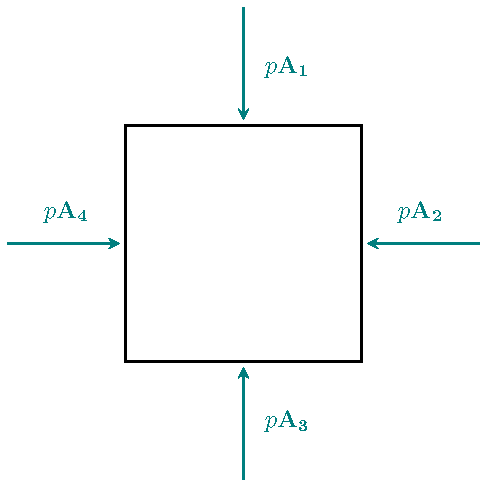
\includegraphics[width=.5\textwidth]{figures/Meshless/pressure_equilibrium.pdf}%
 \caption{
A single volume element surrounded by equal pressure $p$ on each side. The net force it experiences
is the sum of the pressure multiplied by the volumes, surfaces: $\mathbf{F}_{tot} = p \mathbf{A}_1
+
 p \mathbf{A}_2 +  p \mathbf{A}_3 +  p \mathbf{A}_4$. If the vector sum of the surfaces
$\mathbf{A}_j$ doesn't sum up to exactly zero, then the volume element experiences an unphysical
nonzero net force.
 }
 \label{fig:pressure-equilibrium}
\end{figure}


A second very important property of the numerical methods is to ensure that the vector sum of all
cell boundary areas, or in the case of FVPM the effective surfaces between all neighbors, is zero,
i.e.

\begin{align}
 \sum_j \Aijm  =  0 \ .
\end{align}

This condition ensures that no spurious forces and accelerations are being introduced. Consider for
example a fluid which is static and has equal pressure everywhere. Then in the case of a single
volume element, shown in two dimensions in Figure~\ref{fig:pressure-equilibrium}, the net force
experienced by the cell is the sum of the surrounding pressure multiplied by the surface upon which
it acts:

\begin{align}
 \mathbf{F}_{tot} = \sum_j^{\mathrm{all\ surfaces}} p \mathbf{A}_j
\end{align}

If the boundary areas don't have a vector sum of exactly zero, then the net force which the volume
element experiences will also be nonzero. In our example where pressure is equal everywhere, that
is incorrect and unphysical.

It can be shown that the analytical expression for the Ivanova surfaces,
eq.~\ref{eq:IvanovaAij-analytical}, satisfy the closure condition. Using the product rule, we can
write

\begin{align}
 \deldx (\psi_j \psi_i) = \DELDX{\psi_j} \psi_i + \psi_j \DELDX{\psi_i}
\end{align}

and use that to replace the first term in eq.~\ref{eq:IvanovaAij-analytical}:

\begin{align}
   \Aijm &= \int_V \left[ \psi_j \DELDX{\psi_i} - \psi_i \DELDX{\psi_j}  \right] \de V  \\
&= \int_V \left[ \deldx(\psi_j \psi_i) - 2 \psi_i \DELDX{\psi_j}  \right] \de V
\label{eq:closure-midstep}
\end{align}

We can get rid of the first term, $\deldx(\psi_j \psi_i)$, through use of the divergence theorem
once again. The volume integral is transformed into a surface integral:

\begin{align}
    \int_V  \deldx(\psi_j \psi_i) \de V = \int_{\del V} \psi_i \psi_j \hat{\mathbf{n}} \del V
\end{align}

Since we demanded that the partitions of unity have compact support, i.e. $\psi(\x, \x_i, H) = 0 \
\forall \ |\x - \x_i| > H$ and the surface integral is taken along the enclosing surface of the
entire domain, which in general is outside of the compact support radius, the integral evaluates to
zero.

To show that the closure condition holds, we need to show that for some particle $i$ the sum of the
surfaces with all the particles $j$ it interacts with is zero. We now write this sum using the
modifications from eq.~\ref{eq:closure-midstep} and the fact that the first term of
eq.~\ref{eq:closure-midstep} evaluates to zero:


\begin{align}
   \sum_j \Aijm &=
   \sum_j \int_V \left[ \psi_j \DELDX{\psi_i} - \psi_i \DELDX{\psi_j}  \right] \de V  \\
&= \sum_j \int_V \left[- 2 \psi_i \DELDX{\psi_j}  \right] \de V \\
&= \int_V \Bigg[- 2 \psi_i
    \underbrace{\deldx
        \bigg( \underbrace{\sum_j \psi_j}_{= 1} \bigg)
    }_{= 0}
    \Bigg] \de V  = 0
\end{align}


which confirms the closure condition. Note however that this is only valid for the analytical
expression for the Ivanova effective surfaces, not the approximate ones we actually use, given in
eq.~\ref{eq:IvanovaAij}. The approximate ones in general do not satisfy the closure condition
exactly. To demonstrate this, we again take the sum of all effective surfaces over all interacting
particles $j$:

\begin{align}
    \sum_j \Aijm &= \sum_j \left[ V_i \DELDX{\psi_j(\x_i)} - V_j \DELDX{\psi_i(\x_j)} \right] \\
    &=  V_i  \underbrace{
        \deldx \big( \underbrace{\sum_j \psi_j(\x_i)}_{=1} \big)
        }_{= 0} - \sum_j V_j \DELDX{\psi_i(\x_j)}
    = - \sum_j V_j \DELDX{\psi_i(\x_j)}
\end{align}

which in general is non-zero. For it to be exactly zero, we would need a perfectly regular particle
configuration: All volumes $V_j$ need to be equal everywhere, and for every neighboring particle
$j_1$ of particle $i$ there needs to be a neighboring particle $j_2$ which is at the exact same
distance from particle $i$ as $j_1$, but in the exact opposite direction, so that the directions of
the gradients cancel out exactly. This suggests that the method will perform worse when non-regular
particle configurations are present, and may be a hint towards the necessity to employ an
additional scheme to keep the particle configurations somewhat regular throughout the simulation.

As for the Hopkins expression for the effective surfaces \Aij, I am not aware of a general proof
that the closure condition is satisfied. The difficulty in this case is that contrary to the
Ivanova version, we don't have a fully analytical expression readily available, as the approximate
gradient (eq.~\ref{eq:gradient}) is used to obtain the expression. It is however possible to
demonstrate, just like for the Ivanova version, that in a perfectly regular particle configuration
the sum of surfaces is exactly zero.

Assuming a perfectly regular particle configuration leads to all geometry related quantities being
equal:
\begin{itemize}
\item The partition of unity of a particle at a different particle's position is exactly equal to
the second particle's partition of unity at the first particle's position: $\psi_j(\x_i) =
\psi_i(\x_j)$
\item Similarly, all the normalizations at each particle's position, $\omega(\x_i) = \omega$, must
be equal. As a consequence, the particle volumes $V_i = 1 / \omega(\x_i) = V$ are identical as well.
\item All the matrices $\mathcal{E}_i$ (given in eq.~\ref{eq:matrix_E}) are identical, as the sums
$\oldsum_j (\x_j - \x_i)^\alpha(\x_j - \x_i)^\beta$ must be equal everywhere, hence $\mathcal{E}_i
= \mathcal{E}$.
\item As a consequence, the matrices $\mathcal{B} = \mathcal{B}_i = \mathcal{E}_i^{-1}$ are
identical everywhere as well.
\end{itemize}

In this special case, the effective surfaces can be written as

\begin{align}
 \Aijm^\alpha &= V_i \psitilde_j^\alpha(\x_i) - V_j \psitilde_i^\alpha (\x_j) \\
 &= V_i \mathcal{B}_i^{\alpha\beta}(\x_j - \x_i)^\beta \psi_j(\x_i) -
    V_j \mathcal{B}_j^{\alpha\beta}(\x_i - \x_j)^\beta \psi_i(\x_j) \\
 &= V \mathcal{B}^{\alpha\beta}(\x_j - \x_i)^\beta \psi_j(\x_i) -
    V \mathcal{B}^{\alpha\beta}(\x_i - \x_j)^\beta \psi_j(\x_i) \\
 &= 2 V \mathcal{B}^{\alpha\beta}(\x_j - \x_i)^\beta \psi_j(\x_i)
\end{align}

The sum of all surfaces, $\oldsum_j \Aijm$, then vanishes in the case of a perfectly regular
particle configuration (just as was the case for the Ivanova surfaces) because for each neighbor
$j_1$ there is a neighbor $j_2$ for which $(\x_{j1} - \x_i) = -(\x_{j2} - \x_i)$, giving us
$\oldsum_j \Aijm = 0$.












%--------------------------------------------------------------------
\subsection{Conservation of Angular Momentum}\label{chap:meshless-conservation-angular-momentum}
%--------------------------------------------------------------------


To discuss the conservation of angular momentum of the schemes, we will make use of the momentum
equation of the Euler equations without any external forces. Suppose the particles are moving with
some velocity $\mathbf{w} = \DDT{\x}$ be the particle velocity. Then the momentum equation in the
particles' frame of reference is given by (compare eq.~\ref{eq:conservation-law-reference-frame}):

\begin{align}
\deldt (\rho V) + \nabla \cdot \left( \rho \V \otimes (\V - \mathbf{w}) + p \mathds{1} \right) = 0
\end{align}

which we can write component-wise as:

\begin{align}
\deldt (\rho v^\alpha) + \frac{\del}{\del x^\beta} \left( \rho v^\alpha (v^\beta - w^\beta) + p
\delta^{\alpha\beta} \right) = 0
\end{align}

for each spatial component $\alpha$, where the Einstein sum convention over same Greek indices is
assumed again and $\delta^{\alpha \beta}$ is the Kronecker delta. Applying the update formula we
found found for both the Ivanova version (eq.~\ref{eq:meshless-Ivanova}) and the Hopkins version
(eq.~\ref{eq:meshless-Hopkins}), we find for each particle $i$:

\begin{align}
\deldt (V_i \rho_i v_i^\alpha)
= - \sum_j \left( \rho v^\alpha  (v^\beta - w^\beta)  + p \delta^{\alpha\beta} \right)_{ij}
\Aijm^\beta
= \deldt(m_i v_i^\alpha)
\label{eq:angular-momentum-mid}
\end{align}

This expression will be useful to verify whether the angular momentum $\mathbf{L}$ of the
system,

\begin{align}
\mathbf{L} = \sum_i \mathbf{L}_i = \sum_i \x_i \times m_i \V_i
\end{align}

remains constant, where the sum is performed over all particles $i$. To demonstrate whether
$\mathbf{L}$ is constant w.r.t. time, we check that its derivative w.r.t. time is zero:

\begin{align}
\ddt \mathbf{L} &=
    \sum_i \ddt \mathbf{L}_i = \sum_i \ddt \left( \x_i \times m_i \V_i \right) \\
&= \sum_i \left( \DDT{\x_i} \times m_i \V_i + \x_i \times \ddt (m_i \V_i) \right)
\end{align}

To return to the component-wise formulation, we use the three-dimensional Levi-Civita symbol $\epsilon^{\alpha \beta \gamma}$ to express the vector product of the first term:

\begin{align}
\left(\DDT{\mathbf{x}_i} \times \V_i \right)^\alpha &=
    (\mathbf{w}_i \times \V_i)^\alpha =
    \epsilon^{\alpha \beta \gamma} w_i^\beta v_i^\gamma
\end{align}

Similarly, using expression~\ref{eq:angular-momentum-mid}, we can write the second term as:

\begin{align}
\left(\mathbf{x}_i \times \ddt (m_i \V_i)\right)^\alpha &=
\left(\mathbf{x}_i \times - \sum_j \left( \rho \V \otimes (\V - \mathbf{w}) + p
\mathds{1}\right)_{ij} \cdot \mathbf{\mathcal{A}}_{ij} \right)^\alpha \\
&= -\sum_j \epsilon^{\alpha \beta \gamma}  x^\beta
\left( \rho v^\gamma (v^\kappa - w^\kappa) + p \delta^{\gamma\kappa} \right)_{ij} \Aijm^\kappa
\end{align}

giving us:

\begin{align}
\ddt \mathbf{L}_i =
    m_i \epsilon^{\alpha \beta \gamma} w_i^\beta v_i^\gamma
    -\sum_j \epsilon^{\alpha \beta \gamma} x^\beta
        \left( \rho v^\gamma (v^\kappa - w^\kappa) + p \delta^{\gamma\kappa} \right)_{ij}
\Aijm^\kappa
\end{align}

for each particle $i$. Then the derivative w.r.t. time of the entire system is given by:

\begin{align}
\sum_i \ddt \mathbf{L}_i &=
\sum_i \left[
    m_i \epsilon^{\alpha \beta \gamma} w_i^\beta v_i^\gamma
    -\sum_j \epsilon^{\alpha \beta \gamma} x^\beta
        \left( \rho v^\gamma (v^\kappa - w^\kappa)   + p \delta^{\gamma\kappa} \right)_{ij}
\Aijm^\kappa
\right] \\
&=  \epsilon^{\alpha \beta \gamma} \sum_i m_i w_i^\beta v_i^\gamma
-  \epsilon^{\alpha \beta \gamma} \sum_i x_i^\beta \sum_j \left[
   \left( \rho v^\gamma (v^\kappa - w^\kappa)  + p \delta^{\gamma\kappa} \right)_{ij} \Aijm^\kappa
\right]
\end{align}

Making use of our assumption that the flux term $\fc_{ij} = \fc_{ji} = \left( \rho v^\gamma
(v^\kappa - w^\kappa) + p \delta^{\gamma\kappa} \right)_{ij} $ is symmetric in $i$ and $j$, while
the surfaces \Aij are anti-symmetric, and the fact that both summations over indices $i$ and $j$ are over all particles (where we make use of the compact support of the $\psi$ to limit the number of neighboring particles that have a non-zero contribution to the sum over $j$), we can express the
second term as follows:

\begin{flalign}
&\epsilon^{\alpha \beta \gamma} \sum_i x_i^\beta \sum_j \left[
   \left( \rho v^\gamma (v^\kappa - w^\kappa) + p \delta^{\gamma\kappa} \right)_{ij} \Aijm^\kappa
\right] = \\
&\epsilon^{\alpha \beta \gamma} \sum_{i,j} x_i^\beta \left[
   \left( \rho v^\gamma (v^\kappa - w^\kappa) + p \delta^{\gamma\kappa} \right)_{ij} \Aijm^\kappa
\right] = \\
&\frac{1}{2} \cdot 2
\epsilon^{\alpha \beta \gamma} \sum_{i,j} x_i^\beta \left[
   \left( \rho v^\gamma  (v^\kappa - w^\kappa) + p \delta^{\gamma\kappa} \right)_{ij} \Aijm^\kappa
\right] = \\
&\frac{1}{2} \left\{
\epsilon^{\alpha \beta \gamma} \sum_{i,j} x_i^\beta
    \left[ \left(
    \rho v^\gamma  (v^\kappa - w^\kappa) + p \delta^{\gamma\kappa}
    \right)_{ij} \Aijm^\kappa
    \right] +
\epsilon^{\alpha \beta \gamma} \sum_{i,j} x_j^\beta
    \left[ \left(
    \rho v^\gamma  (v^\kappa - w^\kappa) + p \delta^{\gamma\kappa}
    \right)_{ji} \mathcal{A}_{ji}^\kappa
    \right]
\right\} = \\
&\frac{1}{2} \left\{
\epsilon^{\alpha \beta \gamma} \sum_{i,j} x_i^\beta
    \left[ \left(
    \rho v^\gamma  (v^\kappa - w^\kappa) + p \delta^{\gamma\kappa}
    \right)_{ij} \Aijm^\kappa
    \right] -
\epsilon^{\alpha \beta \gamma} \sum_{i,j} x_j^\beta
    \left[ \left(
    \rho v^\gamma  (v^\kappa - w^\kappa) + p \delta^{\gamma\kappa}
    \right)_{ij} \mathcal{A}_{ij}^\kappa
    \right]
\right\} = \\
&\frac{1}{2}
\epsilon^{\alpha \beta \gamma} \sum_{i,j} (x_j^\beta - x_i^\beta)
    \left[ \left(
    \rho v^\gamma  (v^\kappa - w^\kappa) + p \delta^{\gamma\kappa}
    \right)_{ij} \Aijm^\kappa
    \right] = \\
&\frac{1}{2}
\epsilon^{\alpha \beta \gamma} \sum_{i,j} (x_j^\beta - x_i^\beta) (p \Aijm^\gamma) +
\frac{1}{2}
\epsilon^{\alpha \beta \gamma} \sum_{i,j} (x_j^\beta - x_i^\beta)
    \left( \rho v^\gamma  (v^\kappa - w^\kappa) \right)_{ij} \Aijm^\kappa
\end{flalign}


Inserting this expression into our previous findings, we obtain:

\begin{align}
\sum_i \ddt \mathbf{L}_i &=
\epsilon^{\alpha \beta \gamma} \sum_i m_i w_i^\beta v_i^\gamma
-  \epsilon^{\alpha \beta \gamma} \sum_i x_i^\beta \sum_j \left[
   \left( \rho v^\gamma (v^\kappa - w^\kappa)  + p \delta^{\gamma\kappa} \right)_{ij} \Aijm^\kappa
\right] && \\
&= \epsilon^{\alpha \beta \gamma} \sum_i m_i w_i^\beta v_i^\gamma \quad -
&& \text{(i)} \\ \nonumber
& \quad
\frac{1}{2} \epsilon^{\alpha \beta \gamma}
    \sum_{i,j} (x_j^\beta - x_i^\beta) (p \Aijm^\gamma) \quad -
    && \text{(ii)} \\ \nonumber
& \quad
\frac{1}{2} \epsilon^{\alpha \beta \gamma}
    \sum_{i,j} (x_j^\beta - x_i^\beta)
    \left( \rho v^\gamma  (v^\kappa - w^\kappa) \right)_{ij} \Aijm^\kappa
    && \text{(iii)}
\end{align}

For the methods to conserve angular momentum exactly, i.e. $\ddt \mathbf{L} = 0$, two conditions
need to be satisfied. Firstly, the particle velocity $\mathbf{w}$ must be exactly the fluid
velocity: $\mathbf{w} = \V$. This leads to the terms (i) being zero due to the cross product it
contains, as well as term (iii) vanishing.\footnote{
The cancellation of term (iii) due to the condition $\mathbf{w} = \V$ assumes that the expression
for the approximate flux $\fc_{ij} = \left( \rho v^\gamma  (v^\kappa - w^\kappa) \right)_{ij}$
also finds that the approximate factor $(v^\kappa - w^\kappa)_{ij}$ is zero.
That may in general not be the case. However, the second condition required for the total angular
momentum to be conserved, namely the surfaces \Aij to be exactly parallel to distance vector between the particles $i$ and $j$, ensures that the term zeroes out in any case.
}
Secondly, we need the normal vector $\hat{\mathbf{n}}$ of the surfaces $\Aijm =
|\Aijm|\hat{\mathbf{n}}$ to be exactly parallel to the distance vector $\x_j - \x_i$ between any
two particles $i$ and $j$, which leads to the cross product in term (ii) being zero as well. While
we are able to set the particle velocities $\mathbf{w}_i$ as we choose, it is in general not
possible to also enforce that the surfaces are parallel to the distance vector between two particles at all times. This may be the case for exactly regular particle configurations, but not for configurations containing irregularities, as will be shown in
Section~\ref{chap:meshless-comparison}. Hence we must conclude that the methods do not conserve
angular momentum in general.












%=================================================================================
\section{The Full Scheme Applied to the Euler Equations}\label{chap:meshless-full}
%=================================================================================


While the main update formulae for both the Hopkins and Ivanova version of the finite volume
particle methods have been derived, there are still a lot of other points that need to be addressed
in order to obtain a fully functioning method. In what follows, we focus on the application of the
finite volume particle methods on the Euler equations (\ref{eq:euler-equations}). The application
to the moments of the equation of radiative transfer will be discussed in Part~\ref{part:rt}.

Two major points that need to be discussed first are the exact time integration scheme and making
the particles co-move with the fluid. These two topics are intimately linked, as we will see. In
what follows, these topics will be discussed:

\begin{itemize}
 \item Choosing a frame of reference for the flux exchange between two particles
 \item Moving (``drifting'') particles
 \item The time integration scheme
 \item The neighbor search: Finding the smoothing length of particles
 \item Flux limiters for the finite volume particle method
 \item The CFL condition
\end{itemize}

Finally, the full algorithm of the method is presented.







%------------------------------------------------------------------------------------------
\subsubsection{Choosing a Frame of Reference For the Flux Exchange Between Two Particles}
%------------------------------------------------------------------------------------------



The equations that govern the time integration of the states traced by particles give us no
prescription on how to move particles. The Euler equations are Galilei-invariant, and hence are also
valid in co-moving form. So we are basically free to choose to move the particles however we want,
as long as the fluid quantities are correctly transformed into the corresponding frame of reference.
Specifically, the correct frames of reference need to be addressed when the inter-particle fluxes
$\F_{ij}$ of the finite volume particle methods are being computed, as we use the states carried by
the ``left'' and ``right'' particles $i$ and $j$ as left and right states for a Riemann problem. If
each particle's velocity is taken to be the velocity its reference frame, then their states need to
be boosted into a common frame of reference. An obvious choice for a common reference frame is to
take the frame of the ``effective surface'' \Aij. The ``surfaces'' are taken to be at position along
the line connecting particle $i$ and $j$ and at a distance weighted by the respective smoothing
lengths

\begin{align}
    \x_{ij} = \x_i + \frac{h_i}{h_i + h_j} (\x_j - \x_i)
\end{align}

The same weight is used to set the velocity of the surface w.r.t. the rest frame, and hence the
common frame of reference of the particles:

\begin{align}
    \V_{ij} = \V_i + \frac{h_i}{h_i + h_j} (\V_j - \V_i)
\end{align}

where $\V_{i,j}$ are \emph{particle} velocities, which may or may not correspond to the fluid
velocity.

Other choices for the weight to determine the position and velocity of the surfaces are possible,
as long as the resulting term remains anti-symmetric w.r.t. the particles $i$ and $j$. For example,
one could choose to set the surfaces exactly in the middle between both particles. In practice, it
makes little difference in the final results. The smoothing length however is a sensible choice, as
it's a quantity directly related to the local resolution and the local particle number density.

It still remains to determine how to choose the particle velocities. An obvious choice is to move
particles along with the fluid, i.e. to set the particle velocities to the local fluid velocity.
This way the particles, which are also the resolution elements in the scheme, naturally follow the
fluid and the spatial resolution is increased precisely in regions where we need it to be, whereas
``uninteresting'' regions that contain comparatively little material, have small densities, and
generally smooth flows are traced with lower resolution. Other choices are however possible as
well. For example, we could decide not to move the particles at all, which is a neat property of
the finite volume particle methods that we'll make use of to solve the equations of radiative
transfer simultaneously with the Euler equations in Part~\ref{part:rt}.








%-------------------------------------------------------------------
\subsubsection{Time Integration and Particle Drifts}
%-------------------------------------------------------------------

Moving the particles' position is an operation which is usually called a ``drift''. Drift
operations are also commonly used in higher order time integration schemes for particle systems
like the Leapfrog symplectic integrator. The Leapfrog integrator prescribes for a second order
differential equation of the form

\begin{align}
    \frac{\de ^2 x}{\de t ^2} = a && \DDT{x} = v
\end{align}

the following scheme:

\begin{align}
    v_{i+\half} &= v_i + a_i \frac{\Delta t}{2}  && \text{kick} \\
    x_{i+1} &= x_i + v_{i+\half} \Delta t  && \text{drift} \\
    v_{i+1} &= v_{i + \half} + a_{i+1} \frac{\Delta t}{2}  && \text{kick}
\end{align}

Symplectic integrators like the Leapfrog are widely used for their conservational properties. In
particular, they are able to keep bound orbits in N-body systems bounded (i.e.  with a bounded
error in energy), whereas explicit integrators like the Euler integrator or the Runge-Kutta
integrators don't. This means that what physically should be bound orbits can (and will) severely
break energy conservation after a sufficiently high number of integration steps, making what should
be stable systems unstable. Hence the symplectic integrators are preferable.

However, due to the conservational properties of the finite volume particle methods, a full
kick-drift-kick scheme is not strictly necessary. The expressions for the ``effective surfaces''
\Aij (eq.~\ref{eq:HopkinsAij},\ref{eq:IvanovaAij}) are anti-symmetric in particles $i$ and $j$, and
the total flux exchange is thus always conserved. So in the case of hydrodynamics, a simpler
drift-kick scheme suffices, where the ``kick'' operation corresponds to the solution of the update
formulae~\ref{eq:meshless-Hopkins}~and~\ref{eq:meshless-Ivanova}. (Note however that in the case
where gravity is added to the system, the kick-drift-kick scheme becomes necessary once again to
treat the gravitational acceleration adequately.)




%----------------------------------------------------------------
\subsubsection{Obtaining a Time-Centered Problem}
%----------------------------------------------------------------

We can however make use of the drift operation to improve the flux estimates and the order of
accuracy of the scheme. Similarly to how the fluxes between two interacting cells are evaluated at
the midpoint in time between the start and the end of the step in the WAF and the MUSCL-Hancock
schemes (Sections~\ref{chap:WAF}~and~\ref{chap:MUSCL-Hancock}), we can do the same for the finite
volume particle schemes by obtaining the primitive variables (density $\rho$, velocity $v$, and
pressure $p$) at the midpoint in time with the drifts. The inter-particle fluxes in the finite
volume particle schemes are given by the solution to the Riemann problem positioned between two
particles. In turn, the Riemann solvers take the primitive variables as arguments to find the
solution. Hence providing the Riemann solvers with primitive variables advanced in time should allow
us to obtain a better estimate for the inter-particle fluxes throughout the step. To do so, we make
use of the primitive variable formulation of the Euler equations. It is straightforward to show that
the Euler equations can be written in the form

\begin{align}
    \deldt \W + A(\W) \deldx \W = 0 &&
\end{align}

with the primitive state vector $\W$ and Jacobi matrix $A(\W)$

\begin{align}
    \W = \begin{pmatrix}
          \rho \\ v \\ p
         \end{pmatrix}
&&
    A(\W) = \begin{pmatrix}
              v & \rho & 0 \\
              0 & v & 1/\rho \\
              0 & \rho c_s^2 & v
             \end{pmatrix}
\end{align}

Through the general gradient expression \ref{eq:gradient} the gradients of the primitive variables
$\ddx \W$ are available, and so the primitive state $\W^{n+\half}$ at the midpoint in time can be
obtained via

\begin{align}
    \W^{n + \half} &= \W^n - \frac{\Delta t}{2} A(\W) \deldx W
\end{align}








%----------------------------------------------------------------------------
\subsubsection{The Neighbor Search: Determining the Smoothing Length}
%----------------------------------------------------------------------------

Drifting particles has the consequence that the actual particle configuration keeps changing. If a
particle's smoothing length is defined via some requirement for the particle's kernel support radius
to contain an (approximate) number of neighboring particles, it means that after each drift the
smoothing length needs to be re-computed. This process is commonly referred to as a ``neighbor
search'', since determining the smoothing length of each particle also determines which other
particles it will exchange fluxes with. These interaction partners are called neighbors. The
neighbor search is a well known problem in smoothed particle hydrodynamics (see e.g.
\cite{priceSmoothedParticleHydrodynamics2012}) and needs to be solved iteratively using a root
finding technique like the Newton-Raphson or Bisection algorithms due to a circular dependence: If
the smoothing length is defined such that the compact support radius of a kernel includes some given
number of neighbors, then it is related to the local number density of the particles, i.e.

\begin{align}
    h(\x_i) \propto n_i^{1/\nu} \ .
\end{align}

The local number density $n_i = 1/V_i$ on the other hand depends on the associated particle volumes
$V_i$, which in turn require the smoothing length $h$ to be known (see eqs.~\ref{eq:omega}
and~\ref{eq:particle-volume}).

The (average) number of neighbors $N_{NGB}$ which is to be used for a given simulation is in
principle a free parameter. Following the approach of
\citet{dehnenImprovingConvergenceSmoothed2012c}, it can be defined via the parameter $\eta_{res}$:

\begin{align}
    N_{NGB} = V_{S,V} \left( \frac{H}{h} \eta_{res} \right)^\nu \label{eq:number-of-neighbors}
\end{align}

where $V_{S,\nu}$ is the volume of a $\nu$-dimensional sphere, i.e. $2 \pi$ in 2D and $4/3 \pi$ in
3D. The value of the ratio $H/h$ of the compact support radius $H$ to the smoothing length $h$
depends on the kernel choice and dimension. Some values of this ratio for various popular kernels
are given in Table~1 in \citet{dehnenImprovingConvergenceSmoothed2012c}. The default choice for
$\eta_{res}$ is

\begin{align}
    \eta_{res} = 1.2348
\end{align}

which for the cubic spline kernel (eq.~\ref{eq:cubic-spline-kernel}) leads to $\sim 48$ neighbors
in 3D, and $\sim 15$ neighbors in 2D.






%----------------------------------------------------------------------------
\subsubsection{Computing the Gradients}
%----------------------------------------------------------------------------

Once the neighbor search is complete and all smoothing lengths $h$ are known, the gradients
(eq.~\ref{eq:gradient}) can be computed via another sum over all neighboring particles. The
gradients are required to be known before we can proceed with the flux exchanges: While they are
necessary in both the Hopkins and Ivanova version to extrapolate the left and right states at the
``effective surface'' \Aij, the $\psitilde$ terms of \Aij itself in the Hopkins version requires
the gradient terms to be available first. With the gradients being available, the actual
computation of the fluxes and the ``kick'' time integration can be performed with a third sum over
all neighbors, where the sum $\oldsum_j \F_{\alpha, i} \Aijm^\alpha$ is accumulated.




%----------------------------------------------------------------------------
\subsubsection{Flux and Slope Limiters}
%----------------------------------------------------------------------------

Since the finite volume particle methods in this form are second order accurate, we need to employ
limiters in order to prevent spurious oscillations that are a consequence of higher order methods
(see Chapter~\ref{chap:higher-order-schemes}) and to make the scheme total variation diminishing. We
employ the same limiters described by \cite{hopkinsGIZMONewClass2015}. This limiter consists of two
steps: The first step limits the slopes of the individual gradients of each particle. The main idea
is to make sure that if we extrapolate the gradients of a particle to its neighboring particles'
positions, then the extrapolated value shouldn't be higher than the highest actual particle value,
nor lower than the lowest actual value. This prevents new extrema from forming, which is what the
TVD condition requires. So the ``true'' obtained gradient $\nabla \phi^i_{true}$ calculated by use
of eqn. \ref{eq:gradient} of any quantity $\phi^i$ needs to be limited by

\begin{align}
	\nabla \phi_{lim}^i &= \alpha_i \nabla \phi^i_{true} \label{eq:cell-limiter-first}\\
	\alpha_i &= \min\left[ 1, \frac{\phi_{ij\ ngb}^{max} - \phi_i}{\nabla \phi^i_{true} \cdot
r_{max}}, \frac{\phi_i - \phi_{ij\ ngb}^{min}}{\nabla \phi^i_{true} \cdot r_{max}} \right]
\label{eq:cell-limiter-last}
\end{align}


Secondly, to ensure more general stability, a pair-wise slope limiter from
\cite{hopkinsGIZMONewClass2015} is employed during each particle interaction. Unfortunately, only
slope limiting the gradients is not enough to make the method TVD. For a general quantity $Q_k$ of
particle $k$, the slope limited quantity $Q_k^{lim}$ at the intersection $\mathbf{x} =
\mathbf{x}_{kl}$ for the interaction between this particle $k$ and some other particle $l$ is

\begin{equation}
	Q_k^{lim} =
	\begin{cases}
		Q_k
						& \text{ if } Q_k = Q_l \\
		\max\left\{ Q_-,
			\min\{ \overline{Q}_{kl} + \delta_2, Q_k + \DELDX{Q_k} (\mathbf{x}_{kl} -
\mathbf{x}_k)\}
		\right\}
						& \text{ if } Q_k < Q_l \\
		\min\left\{ Q_+,
			\max\{ \overline{Q}_{kl} - \delta_2, Q_k + \DELDX{Q_k} (\mathbf{x}_{kl} -
\mathbf{x}_k)\}
		\right\}
						& \text{ if } Q_k > Q_l
	\end{cases}  \label{eq:face-limiter-first}
\end{equation}


where


\begin{align}
Q_- &=
	\begin{cases}
		Q_{min} - \delta_1
						& \text{ if } \mathrm{sign} (Q_{min} - \delta_1) = \mathrm{sign} (Q_{min})\\
		\frac{Q_{min}}{1 + \delta_1 / | Q_{min}|}
						& \text{ if } \mathrm{sign} (Q_{min} - \delta_1) \neq \mathrm{sign}
(Q_{min}) \\
	\end{cases}\\
%
Q_+ &=
	\begin{cases}
		Q_{max} + \delta_1
						& \text{ if } \mathrm{sign} (Q_{max} + \delta_1) = \mathrm{sign} (Q_{max})
\\
		\frac{Q_{max}}{1 + \delta_1 / | Q_{min}|}
						& \text{ if } \mathrm{sign} (Q_{max} + \delta_1) \neq \mathrm{sign}
(Q_{max}) \\
	\end{cases}\\
%
\overline{Q}_{kl} &=
	Q_k + \frac{|\mathbf{x}_{kl} - \mathbf{x}_{k}|}{|\mathbf{x}_{l} - \mathbf{x}_{k}|} (Q_l -
Q_k)\\
%
Q_{min} &= \min\{ Q_k, Q_l \} \\
Q_{max} &= \max\{ Q_k, Q_l \} \\
\delta_1 &= \gamma_1 | Q_k - Q_l | \\
\delta_2 &= \gamma_2 | Q_k - Q_l |  \label{eq:face-limiter-last}
\end{align}

where $\gamma_1$ and $\gamma_2$ are free parameters, the recommended choice being $\gamma_1 =
1/2$, $\gamma_2 = 1/4$.









%-------------------------------------------------
\subsubsection{The CFL Condition}
%-------------------------------------------------

The final point left to be discussed is the determination of the time step size of individual
particles. A ``cell size'' $\Delta x$ of  a particle is estimated using

\begin{align}
    \Delta x \approx \left(\frac{V_i}{V_{S,\nu}} \right)^{1/\nu}
\end{align}

where $V_{S,\nu}$ is the volume of a $\nu$-dimensional unit sphere, so $4/3 \pi$ in 3D. The signal
velocity is estimated as

\begin{align}
    v_{i,sig} = \max \{ |v_{i,fluid} - v_{i,particle}| + c_{s,i}, c_{s,i} + c_{s,j} \} \ .
\end{align}

We take the velocity difference between the fluid and the particle, since that is the velocity at
which the fluid in the co-moving frame with the particle would propagate, and the sound speed $c_s$
to estimate the propagation velocity of the emanating waves of the Riemann problem, similar to
the suggested estimate for Godunov's method, eq.~\ref{eq:wavespeed-estimate-godunov}. To ensure
that no problems arise in cases where two particles approach each other, the additional
upper boundary of the sum of the wave speeds $c_{s,i} + c_{s,j}$ for particle $i$ and all its
neighbors $j$ is added. This leads to the time step estimate

\begin{align}
    \Delta t = C_{CFL} \frac{\Delta x}{v_{sig}} \label{eq:meshless-cfl}
\end{align}

Typically a safe choice of $C_{CFL} \lesssim 0.4$ is recommended.








%-------------------------------------------------
\subsubsection{The Full Algorithm}
%-------------------------------------------------

To conclude this Section, let's explicitly write down the algorithm to solve the Euler Equations
from some $t_{start}$ to some $t_{end}$ using the full kick-drift-kick Leapfrog integration scheme:

\algo{Evolving The Euler Equations From $t_{start}$ to $t_{end}$ Using Finite Volume Particle
Methods}
{
To start, set $t_{current} = t^0 = t_{start}$ and set up the initial states $\U_i^0$ for
each particle $i$.\\[.5em]
%
While $t_{current} < t_{end}$, solve the $n$-th time step:\\[.5em]
%
\indent~~~~Find the maximal permissible time step $\Delta t$ using
eq.~\ref{eq:meshless-cfl}.\\[.5em]
%
\indent~~~~Kick the particles: Update the the particle velocity (not the fluid velocity) \\
\indent~~~~over the time step $\Delta t / 2$.\\[.5em]
%
\indent~~~~Drift the particles: Move their positions over the time step $\Delta t$.\\[.5em]
%
\indent~~~~Obtain the primitive variables at the midpoint in time, $\W_i^{n+\half}$.\\[.5em]
%
\indent~~~~Do a ``neighbor search loop'' over neighboring particles, and determine\\
\indent~~~~the smoothing length $h$ for all particles $i$.\\[.5em]
%
\indent~~~~Do a ``gradient loop'' over neighboring particles to determine the gradients\\
\indent~~~~of the primitive variables for each particle.\\[.5em]
%
\indent~~~~Do a ``flux exchange loop'' over neighboring particles, during which all\\
\indent~~~~neighboring particles $i$, $j$ interact with each other:\\[.5em]
%
\indent~~~~~~~~For each particle pair $i$, $j$, compute the ``effective surfaces'' \Aij.\\[.5em]
%
\indent~~~~~~~~Find the position $\x_{ij}$ and velocity $\V_{ij}$ of the \Aij.\\[.5em]
%
\indent~~~~~~~~Boost the primitive variables $\W^{n+\half}$ to the common reference frame \\
\indent~~~~~~~~with velocity $\V_{ij}$, and extrapolate them using gradients at the position
$\x_{ij}$.\\[.5em]
%
\indent~~~~~~~~Use the boosted and extrapolated states to find the inter-particle fluxes by \\
\indent~~~~~~~~solving the Riemann problem. Accumulate the sum of all fluxes for each \\
\indent~~~~~~~~particle, boosted back into the frame of reference of the respective
particle.\\[.5em]
%
\indent~~~~Obtain the updated states $\U_i^{n+1}$ using eq.~\ref{eq:meshless-Hopkins-explicit} over
the time step $\Delta t$.\\[.5em]
%
\indent~~~~Kick the particles again: update the particle velocities over the time step $\Delta
t/2$.\\[.5em]
%
\indent~~~~Update the current time: $t_{current} = t^{n+1} = t^n + \Delta t$ \\
}


Note that in the absence of external forces like gravity the first kick operation is unnecessary,
while the second kick operation consists of directly setting the particle velocities to the fluid
velocities (assuming the particles are treated as exactly Lagrangian, without any corrections or
modifications). Including external acceleration terms however makes the first kick operation
necessary again.








%--------------------------------------------------------------------
\section{Individual Timstepping}\label{chap:individual-timesteps}
%--------------------------------------------------------------------



\begin{figure}
 \centering
 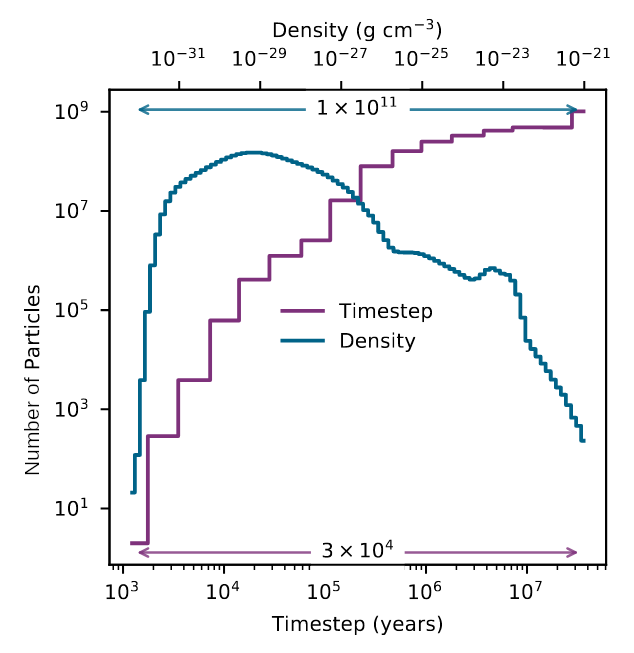
\includegraphics[width=.5\textwidth]{figures/Meshless/EAGLE_timesteps.png}
 \caption{
Histogram of particle time steps and densities from the EAGLE simulation suite
\citep{schayeEAGLEProjectSimulating2015, schallerEAGLESimulationsGalaxy2015} at redshift $z = 0.1$,
where galaxies are fully formed.
With the density spanning 11 orders of magnitude, the resulting time step sizes for particles span
four orders of magnitude. Only a small minority of particles has very small time steps, motivating
the approach to allow particles to be integrated according to their individual time step sizes
rather than limiting all particles to the globally minimal time step size. \\
%
This figure is adapted from \cite{borrowSWIFTMaintainingWeakscalability2018} with permission from
the author.
}
 \label{fig:eagle-timesteps}
\end{figure}





A huge challenge in cosmological simulations is the extreme range of states that are present. For
example, the EAGLE simulation \citep{schallerEAGLESimulationsGalaxy2015}, shown in
Figure~\ref{fig:eagle-timesteps}, reports ranges in particle densities of $11$ orders of magnitude,
and $6$ orders of magnitudes in internal energies. We can make an estimate how that will affect
time step sizes: For the ``cell size'' $\Delta x$ (in 3D), we can use:

\begin{align}
\Delta x \sim V_i^{1/3} = (m_i/\rho_i)^{1/3} \propto \rho_i^{-1/3} \ .
\end{align}

For the propagation speed $v_{sig}$, we can use the approximation of the local sound speed, i.e.

\begin{align}
v_{sig} \sim c_{s} = \sqrt{p/\rho} = \sqrt{u (\gamma - 1)} \propto  u^{1/2} \ .
\end{align}


giving us the estimate

\begin{align}
\Delta t \propto \frac{\Delta x}{v_{sig}} \propto u^{-1/2} \rho^{1/3}
\end{align}

which leads to about 4 orders of magnitude in time step size differences. Additionally,
Figure~\ref{fig:eagle-timesteps} also shows that only a minority of particles will have small time
step sizes. If we were to use a global time step size throughout the simulation, i.e. limit the
time step of all particles by the globally minimal time step size, it would mean that the majority
of the particles is restricted to a much smaller time step size than their individual CFL-condition
would allow for. It would also mean that the simulation would require several orders of magnitude
more steps than strictly necessary if it weren't for the minority of particles with very small time
steps. This additional expense would make cosmological simulations prohibitively expensive.

To circumvent this issue, it is necessary to allow particles to have individual time step sizes,
albeit with some restrictions. Particles are given time step sizes based on their individual CFL
condition, rounded down to a power-of-two fraction of the maximal time step size of the system
$t_{max}$:

\begin{align}
    \Delta t_i = \frac{t_{max}}{2^n}
\end{align}

with $n \geq 0$. The maximal time step size of the system is typically the requested time from
beginning to end of the simulation. Allowing only specific values for time step sizes of particles
is akin to histogramming their time step sizes, and $n$ is typically referred to as the ``time
bin'' of the particles. The absolute minimal time step size is given by $t_{min} = t_{max} /
2^{N_{bins}}$, where $N_{bins}$ is the total number of available time bins. This method has been
used in SPH simulations since \citet{hernquistTREESPHUnificationSPH1989}.

The entire simulation progresses by advancing the current simulation time by a time step size which
is a power-of-two multiple of $t_{min}$. The system time step size is still determined by the
minimal global time step, but only the particles that require such a small time step are also
updated. This is schematically shown in Figure~\ref{fig:individual-timesteps}. Whether a particle
needs to finish its time integration on the current simulation step is then determined by whether
the current simulation time divided by the particle's time step has a modulo of zero. Since
particles have time step sizes which are always a power-of-two apart from each other, this means
that at each simulation step, there is a maximal time bin $m$ for which the division of the current
system time with $m$ gives modulo of zero, and all particles with time bin $n \leq m$ will require
an update in that simulation step, as can be seen in Figure~\ref{fig:individual-timesteps}.

With particles being allowed to have individual time steps, the update formula for the finite volume
particle methods (eq.~\ref{eq:meshless-Hopkins-explicit}) needs to be slightly updated in order to
maintain its conservative properties. In particular, rather than exchanging fluxes, particles now
need to exchange time integrated fluxes:

\begin{align}
\U_i^{n+1} =
    \U_i^n + \frac{1}{V_i} \sum_j \min\{ \Delta t_i, \Delta t_j \} \F_{\alpha, ij} \Aijm^\alpha
\label{eq:meshless-explicit-individual-timesteps}
\end{align}

The time integration needs to be the smaller of the two time step sizes $\{\Delta t_i,\  \Delta
t_j\}$ since if one particle has a smaller time step size than the other, it also means that there
will be several interactions between that particle pair, each with the time step size of the smaller
of the two. This ensures that the total exchange of fluxes remains conservative, as the fluxes
``removed'' from particles $j$ remain exactly equal to the fluxed ``added'' to particle $i$. If some
neighboring particles $j$ have smaller time steps than particle $i$, then the net sum of the fluxes
is accumulated during the exchanges and applied only once at the point where particle $i$ is being
updated again.





\begin{figure}
 \centering
 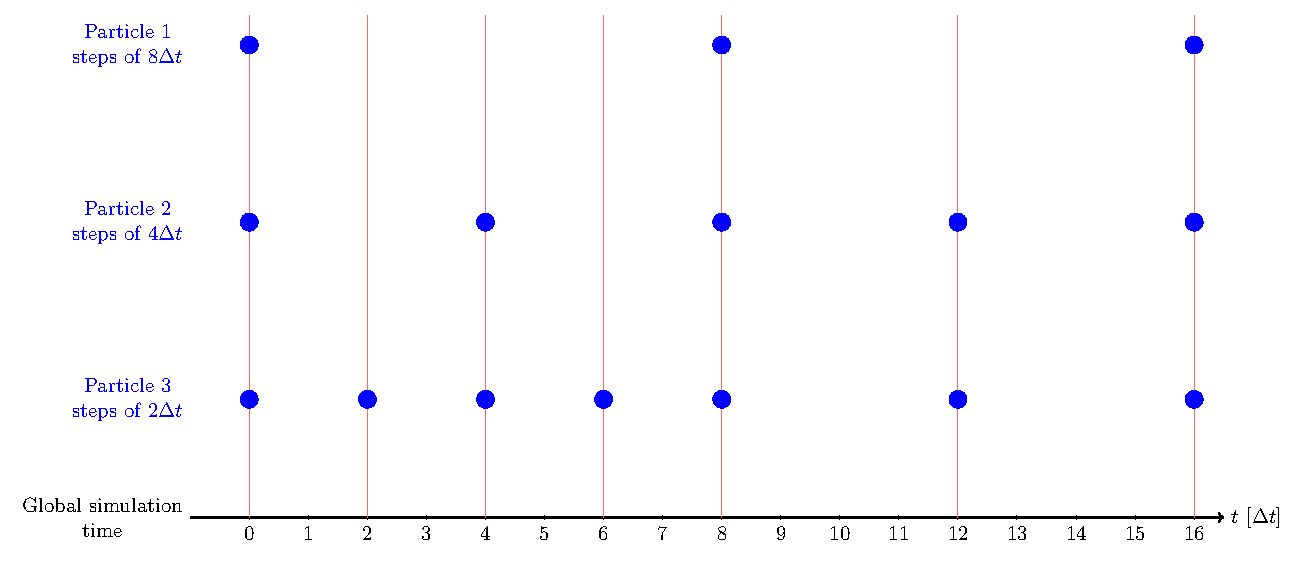
\includegraphics[width=\textwidth]{figures/Meshless/individual_timestepping.pdf}
 \caption{
Illustration of the individual time stepping scheme. Three particles with initially different time
step sizes $2 \Delta t$, $4 \Delta t$, and $8 \Delta t$, respectively, are shown, where $\Delta t$
denotes a minimal time steps size. The simulation progresses by advancing the time according to the
global minimal time step size, which in the beginning is $2 \Delta t$. Each simulation step is
marked as a red line. Since in this example there are no particles with time step size of $\Delta
t$, all times that are an odd integer multiple of $\Delta t$ are skipped over.
At each simulation step, only particles for which the current simulation time divided by the time
step size has a modulo of zero are being updated.\\
%
In this illustration, particle 3 changes its time step size at the at the simulation time $t = 8
\Delta t$ from $2 \Delta t$ to $4 \Delta t$ for reasons which are unimportant. From that point, the
simulation step can be increased to $4 \Delta t$, and fewer total number of simulation steps are
necessary.
}
 \label{fig:individual-timesteps}
\end{figure}


























%=================================================================================
\section{Comparing the ``Hopkins'' and ``Ivanova'' Versions}\label{chap:meshless-comparison}
%=================================================================================

With the full method presented in Section~\ref{chap:meshless-full}, we can now turn to comparing
the ``Hopkins'' and ``Ivanova'' versions of the methods.
The difference between the Hopkins version and the Ivanova version of the finite volume particle
method lies in the expression for the ``effective surface'' \Aij. These surfaces are rather abstract expressions, and it seemed worthwhile to invest time to investigate how they behave, how they can be interpreted, and to see whether there might be significant differences between the two versions.












%------------------------------------------------------------------------
\subsection{Behavior of the Effective Surfaces}
%------------------------------------------------------------------------

Let's begin with the behavior of the effective surfaces without looking into their application on
evolving problems in time just yet. To compute and visualize their behavior of these effective
surfaces, I have developed a dedicated Python package named \mbox{\codename{astro-meshless-surfaces}},
which is publicly available on
\href{https://github.com/mladenivkovic/astro-meshless-surfaces}{PyPI.org} and on
\url{https://github.com/mladenivkovic/astro-meshless-surfaces}.




%-----------------------------------------------------------------------
\subsubsection{Differences in Direction and Magnitude of the \Aij}
%-----------------------------------------------------------------------

Figure \ref{fig:uniform-arrows} shows the effective surfaces of both versions for a central
particle in a uniform particle distribution, while Figure \ref{fig:perturbed-arrows} shows them for
a non-uniform particle configuration. The surfaces are drawn as (pseudo-)vectors starting at the
position

\begin{equation}
	\x_{ij} = \x_i + \frac{h_i}{h_i + h_j}(\x_j - \x_i)		\label{eq:xij}
\end{equation}

which is the position where the effective surfaces would be ``placed'' during the flux exchange of
the particles. Only the particles within the compact support radius of the central particle are
shown.

\begin{figure}[htpb]
\centering
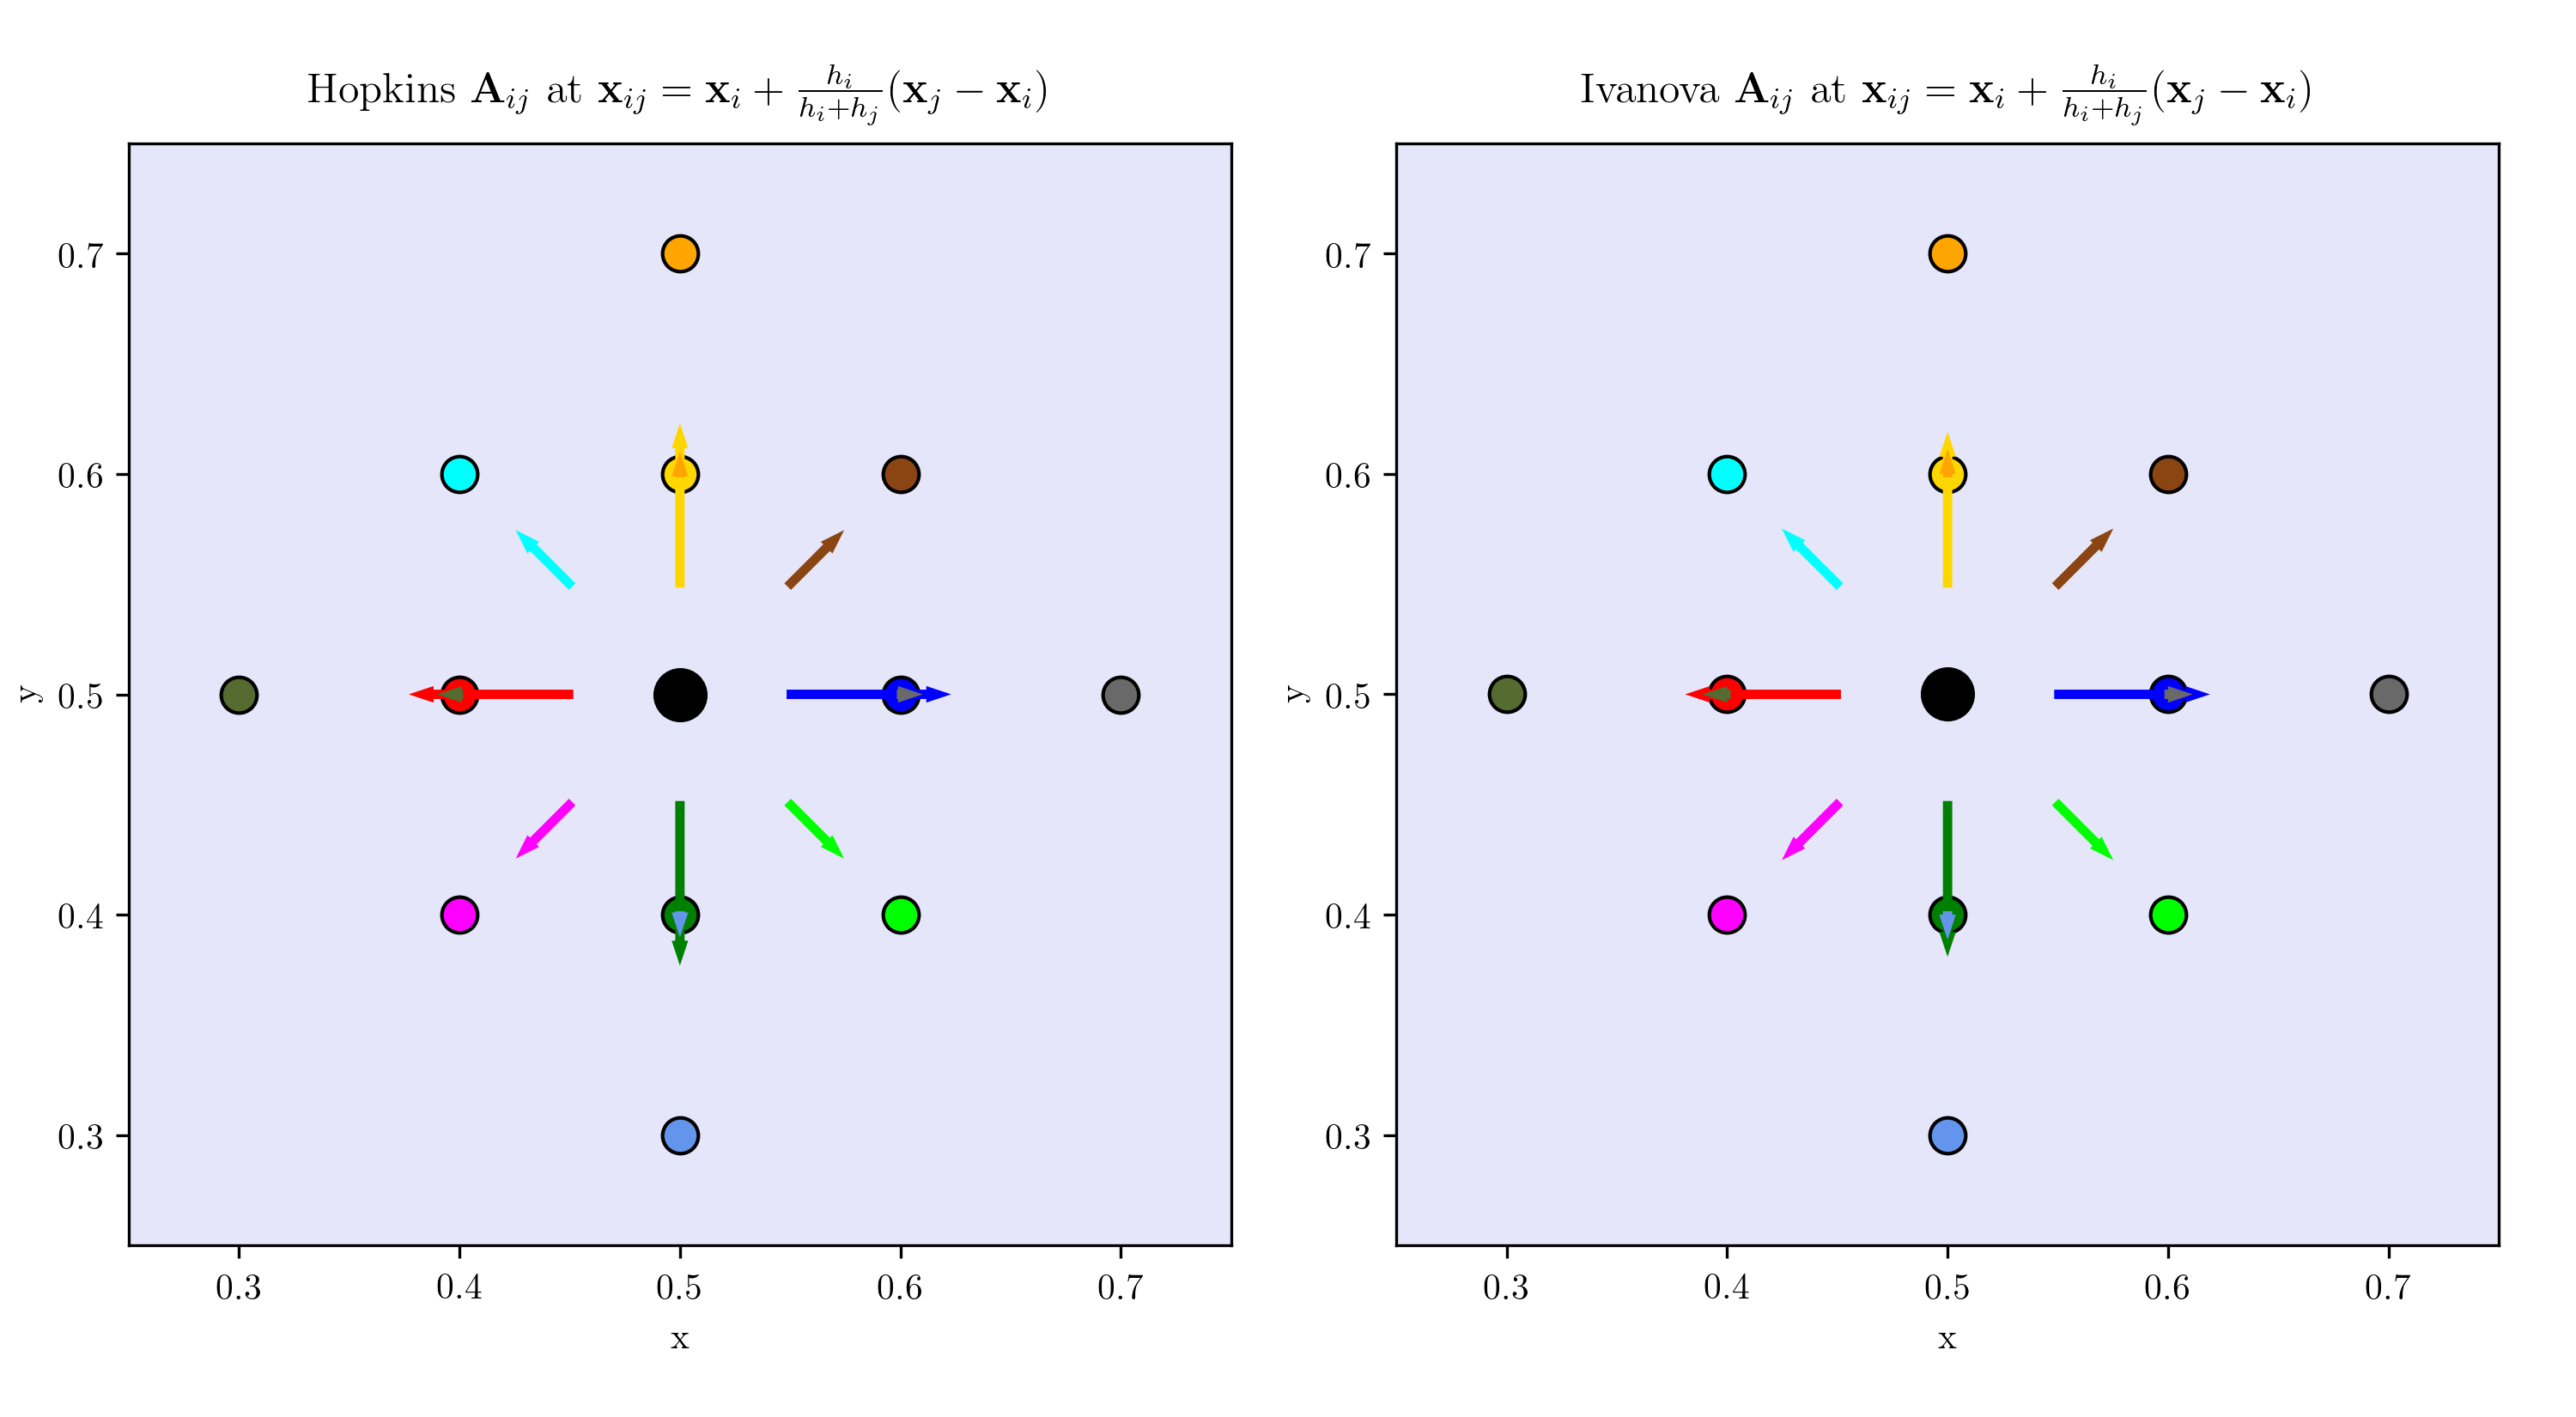
\includegraphics[width=\textwidth]{figures/Meshless/effective-area-hopkins-vs-ivanova.png}
\caption{\label{fig:uniform-arrows}
    The effective surfaces \Aij\ for the Hopkins and Ivanova expression for the black particle in a
    uniform particle distribution.  Only the particles within the compact support radius of the
    central particle are plotted.
}
\end{figure}



\begin{figure}[htpb]
\centering
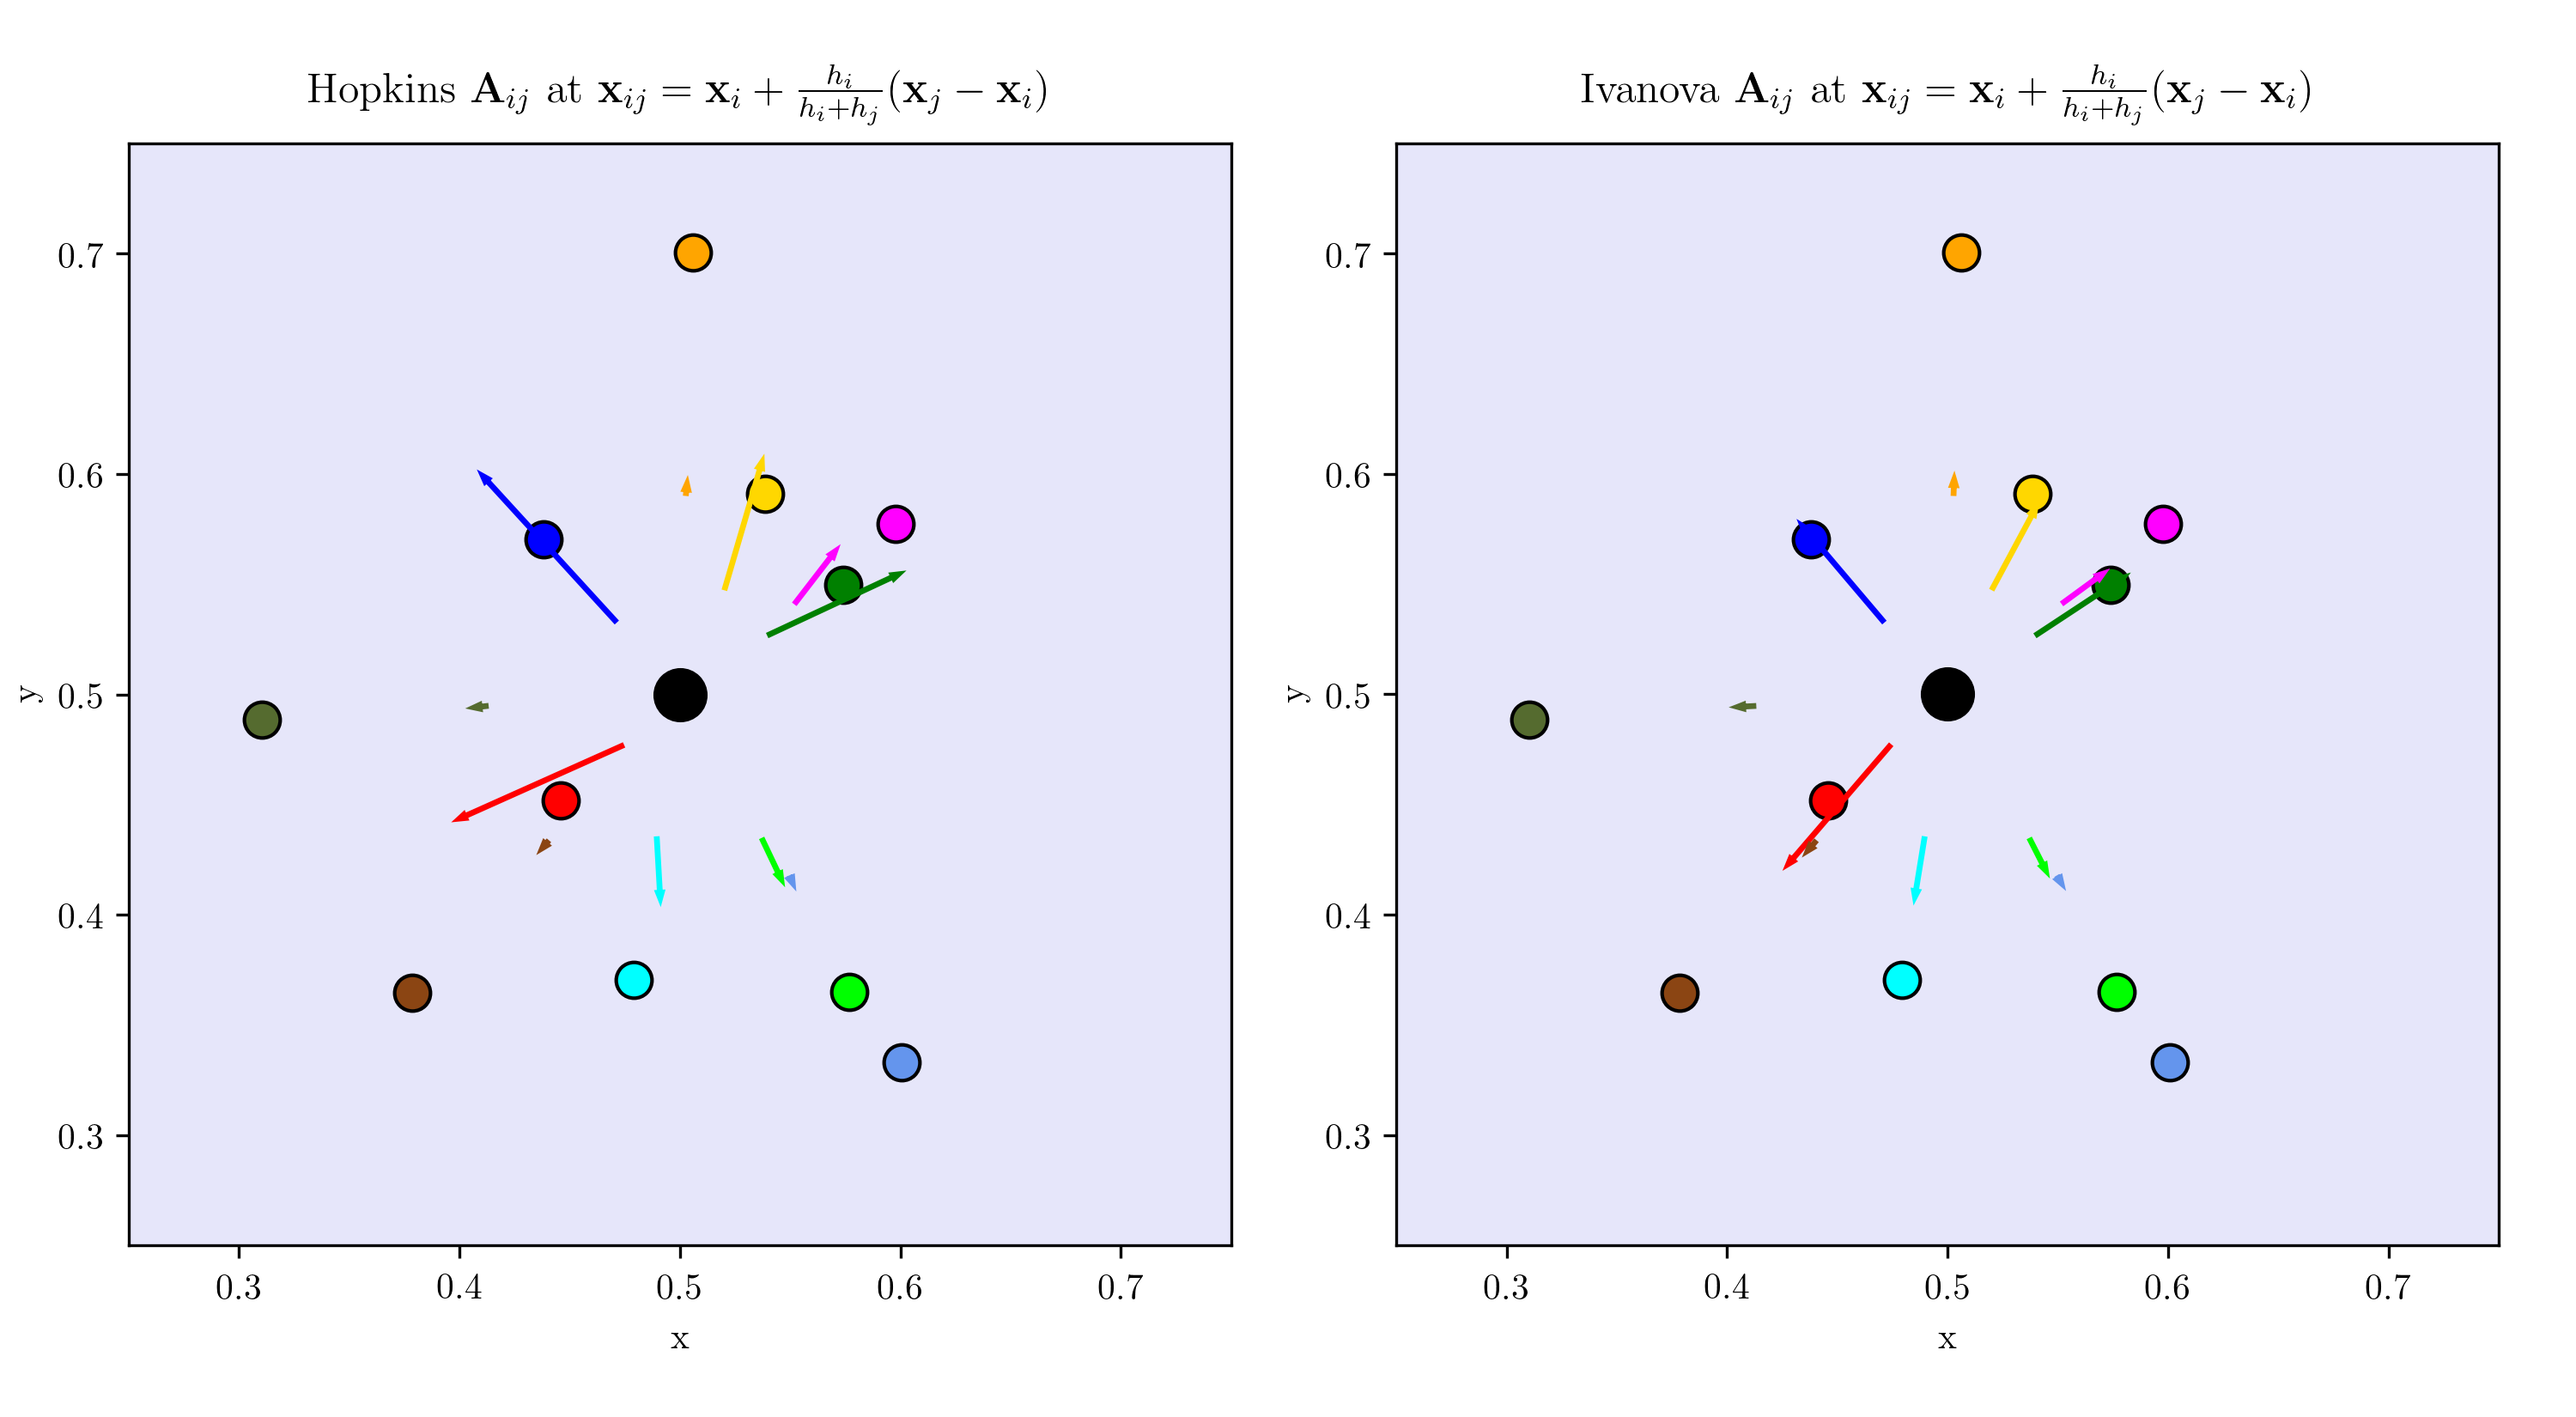
\includegraphics[width=\textwidth]{
figures/Meshless/effective-area-hopkins-vs-ivanova-perturbed.png}
\caption{\label{fig:perturbed-arrows}
    The effective surfaces \Aij\ for the Hopkins and Ivanova expression for the black particle
    in a non-uniform particle distribution. Only the particles within the compact support radius of
    the central particle are plotted.
}
\end{figure}

Comparing the norm of the \Aij\ between the Hopkins and the Ivanova version for the same
neighboring particles, the ratio of the Hopkins over Ivanova lengths varies between 1.06 and 0.33
for the uniform case and between 1.60 and 0.28 for the non-uniform case.
The ratio tends to lower values with increasing neighbor particle distance.

In the non-uniform particle distribution a striking feature is that the effective surfaces do not
point towards the neighboring particle which they are associated with.
In the Hopkins formulation, the reason for that is that the $\psitilde$ (eq. \ref{eq:psitilde}) in
the expression for \Aij have a non-zero contribution from other dimensions. These contributions
enter through the matrix multiplication, and occur even in the case where the two interacting
particles are positioned along a line parallel to the coordinate axes.
As for the Ivanova case, the direction of $\nabla \psi$ will in general not be radially symmetric,
as $\psi(\x)$ is also not radially symmetric in general (see Figure~\ref{fig:psi-of-x-contour}).




%-----------------------------------------------------------------------
\subsubsection{Checking the Closure Condition}
%-----------------------------------------------------------------------

A further check that can be made is to verify whether the closure condition (see
Section~\ref{chap:meshless-conservation-closure}), i.e. $\oldsum_j \Aijm = 0$, is satisfied. In the
uniform particle configuration this is satisfied to machine precision. In the non-uniform case
however, both expressions sum up to a value around the same order of magnitude of a single \Aij,
which tends to be $\approx 10^{-3} - 10^{-4}$. The effect remains for higher particle numbers and
higher neighbor numbers used, i.e. the magnitude of both the \Aij\ and the sum over all \Aij\ for an
individual particle decrease, but their ratio remains about the same. It should be noted that in any
case investigated, the $\oldsum_j \Aijm = 0$ for the Ivanova expression was closer to zero by about
one order of magnitude, but also the total sum of the norms of all \Aij, $\oldsum_j |\Aijm|$, of the
Ivanova version was in every case smaller than the one for the Hopkins version.










%-----------------------------------------------------------------------
\subsubsection{\Aij as a Function of Neighbor Position}
%-----------------------------------------------------------------------

Let us now look into how the effective surfaces between two particles behave when one particle's
position is varied. To examine that, a particle is placed in an otherwise uniform configuration and
the \Aij\ are computed at that place with respect to the central particle. Figure
\ref{fig:displaced-particle} shows the x- and y- component of \Aij\ and $|\Aijm|$ for both
discretization methods. The obtained value is plotted at the particle's position. Note that in
during the actual flux exchanges the effective surface would be assumed to be in a different place
than is currently plotted, namely at the position specified by eq. \ref{eq:xij}.


As one would expect, the \Aij point towards the central particle and increase with distance until
another particle becomes too close and starts having a bigger contribution via the $\psi(\x)$ at
that position. The Hopkins \Aij reach higher peak values, and the contour shapes aren't perfect
circles, but a little ``boxy''. In accordance to the findings of the direct comparison in the
previous section, the Ivanova methods display a higher relative contribution with increasing
distance from the central particle. The same behavior of the effective surfaces pertains for varying
choices of neighbor number per particle, and for different kernels.



\begin{figure}[htpb]
	\centering
	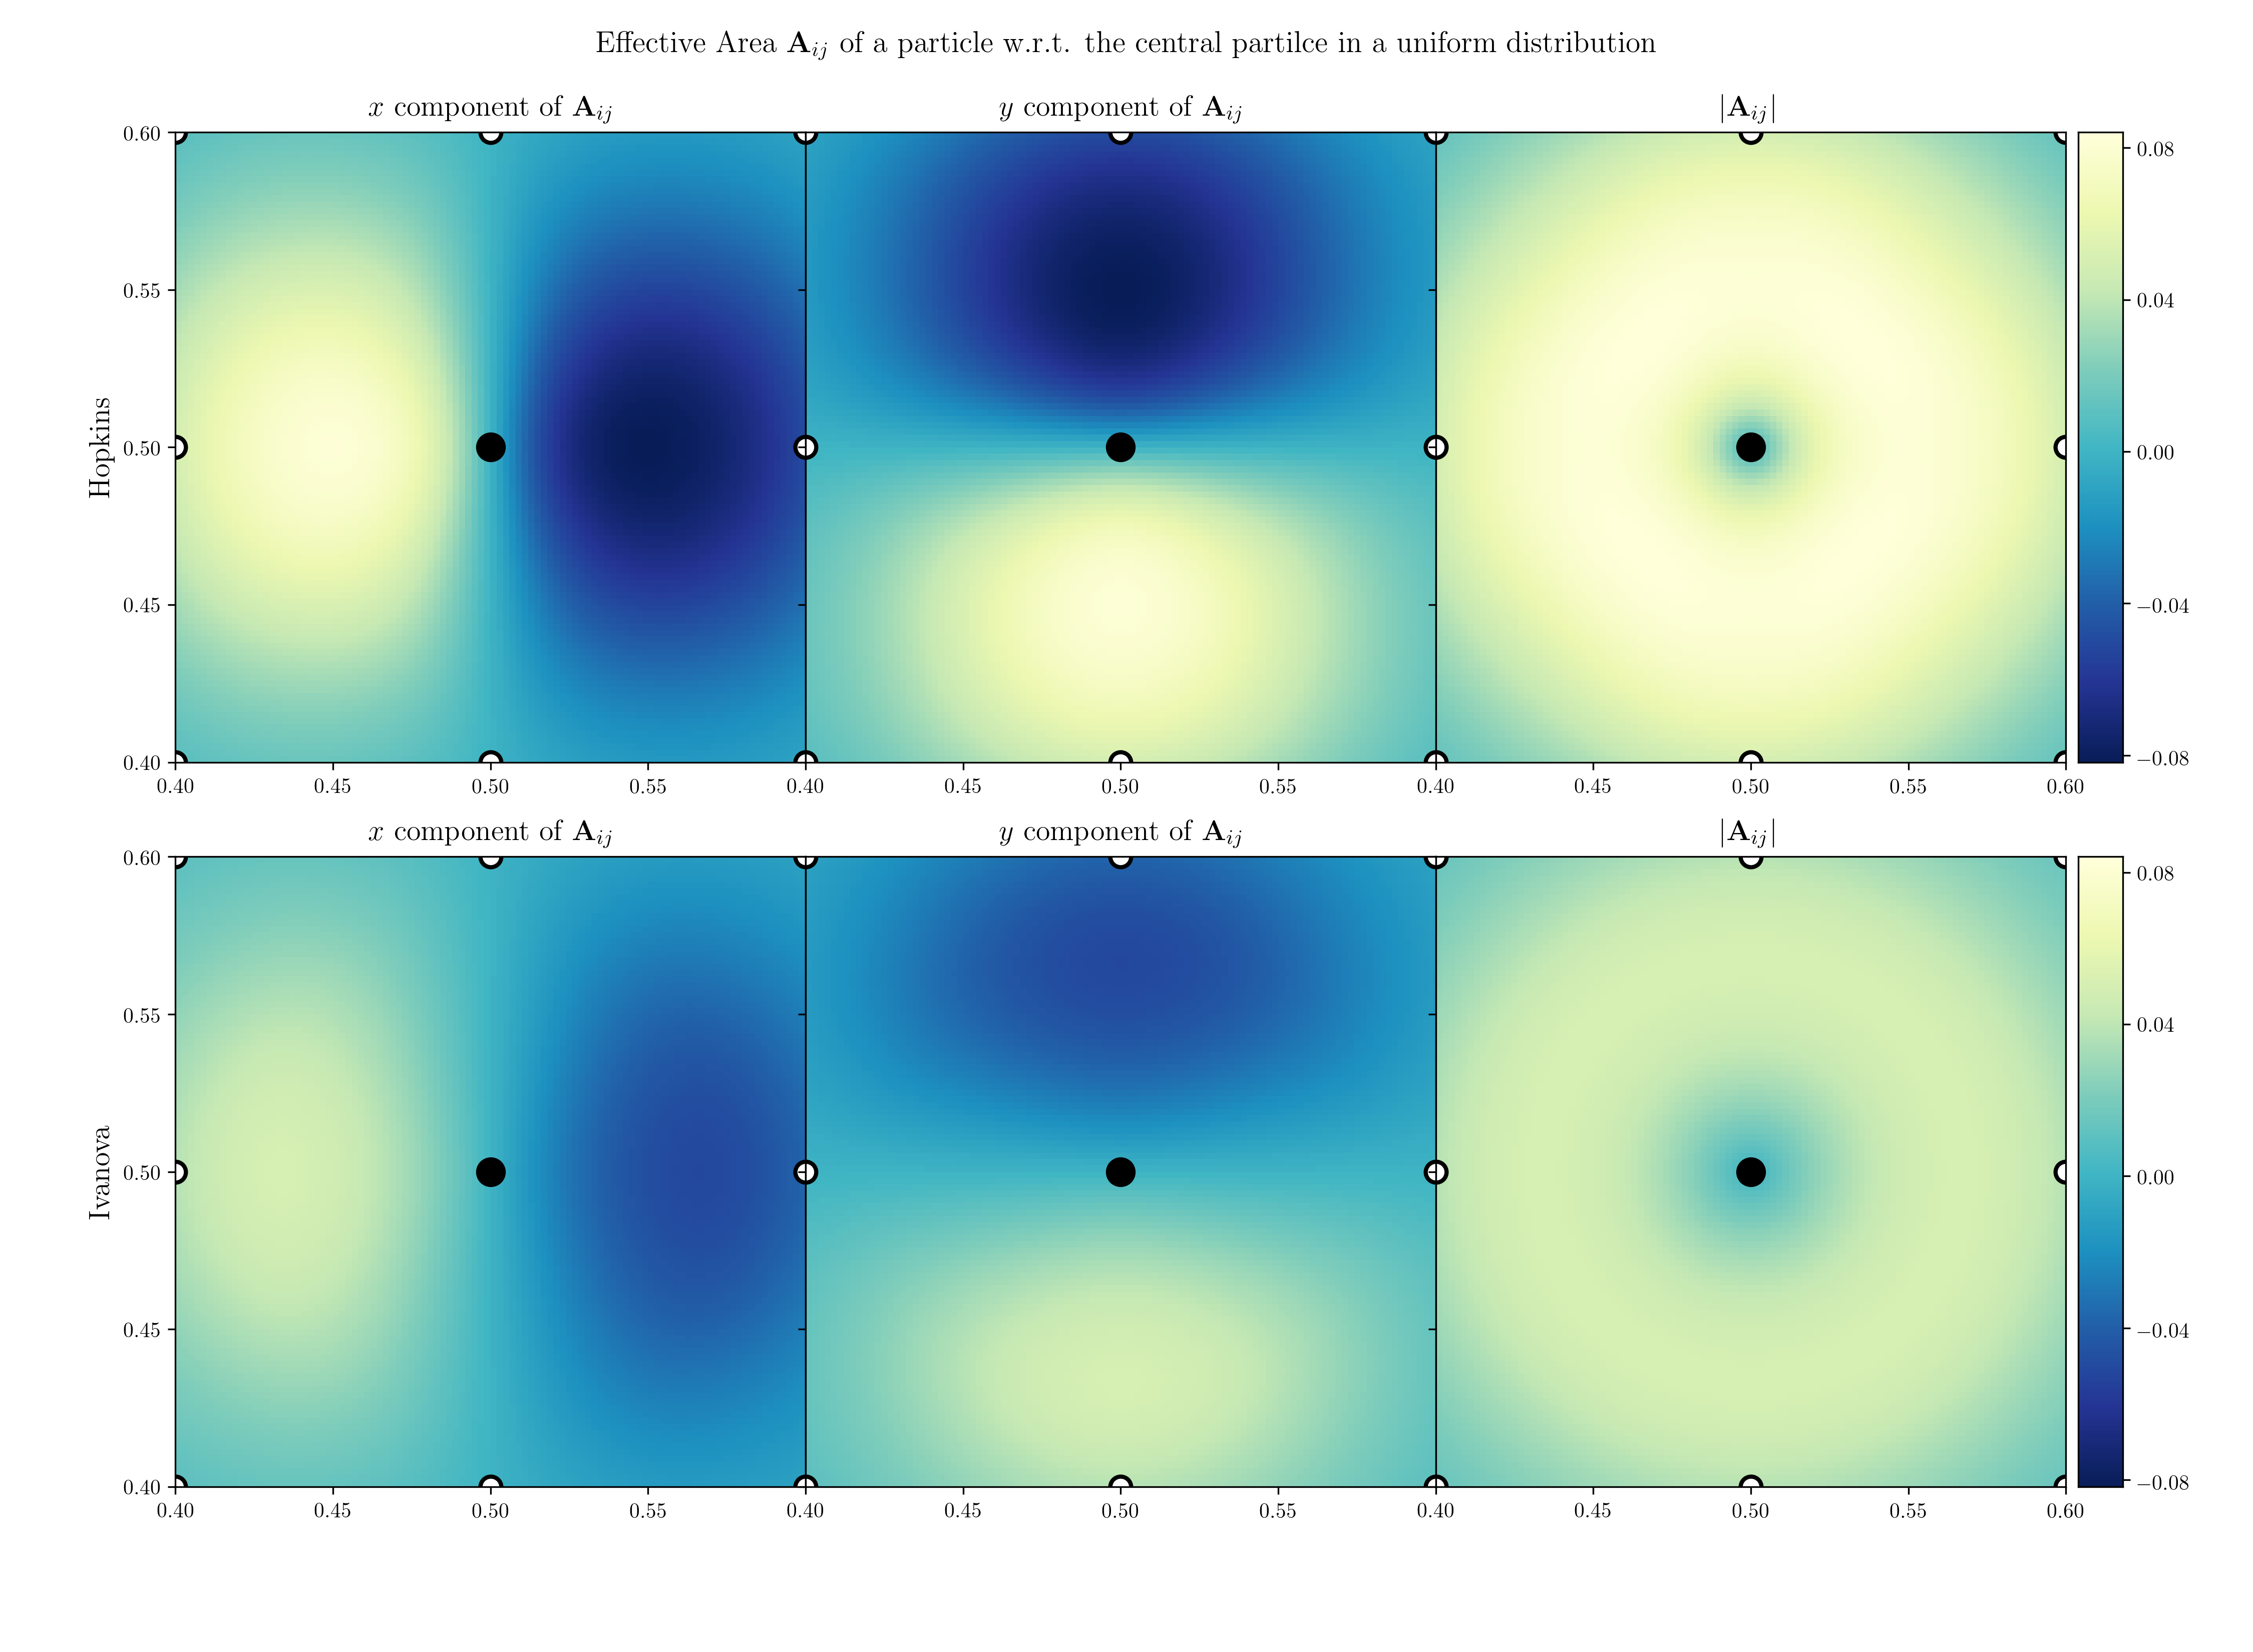
\includegraphics[width=\textwidth]{figures/Meshless/effective-area-displaced-particle.png}
	\caption{\label{fig:displaced-particle}
		x-component, y-component, and norm of \Aij\ for both the Hopkins and Ivanova expression for
a particle being displaced in an otherwise uniform particle configuration w.r.t the central (black)
particle.
		The white circles show the positions of the closest neighbor particles of the central one.
		The value of \Aij\ of the displaced particle at a certain point on the plotted plane
determines that point's color.
	}
\end{figure}














%-------------------------------------------------------------
% \subsubsection{Dependence on smoothing lengths and kernels}
%-------------------------------------------------------------

% Figure \ref{fig:different-smoothing-lengths} shows the \Aij\ for both the Hopkins and Ivanova
% expressions for an additional particle within a uniformly distributed particle grid for varying
% resolution parameters $\eta$ as factors of $\eta_0 = 1.2348$.
% $\eta$ determines the number of neighbors and thus the resolution of the computations. The average
% number of neighbors can be obtained in 2D with
%
% \begin{align}
% 	N_{ngb} = \pi \left(\frac{H}{h} \eta \right)^2 \approx 15 \text{ for } \eta = 1.2348
% \end{align}
%
% The norm of the computed \Aij\ is plotted at that displaced particles' position. With decreasing
% smoothing lengths, the ``boxy'' contour shapes are easier to spot.
%
%
% \begin{figure}[htpb]
% \centering
% 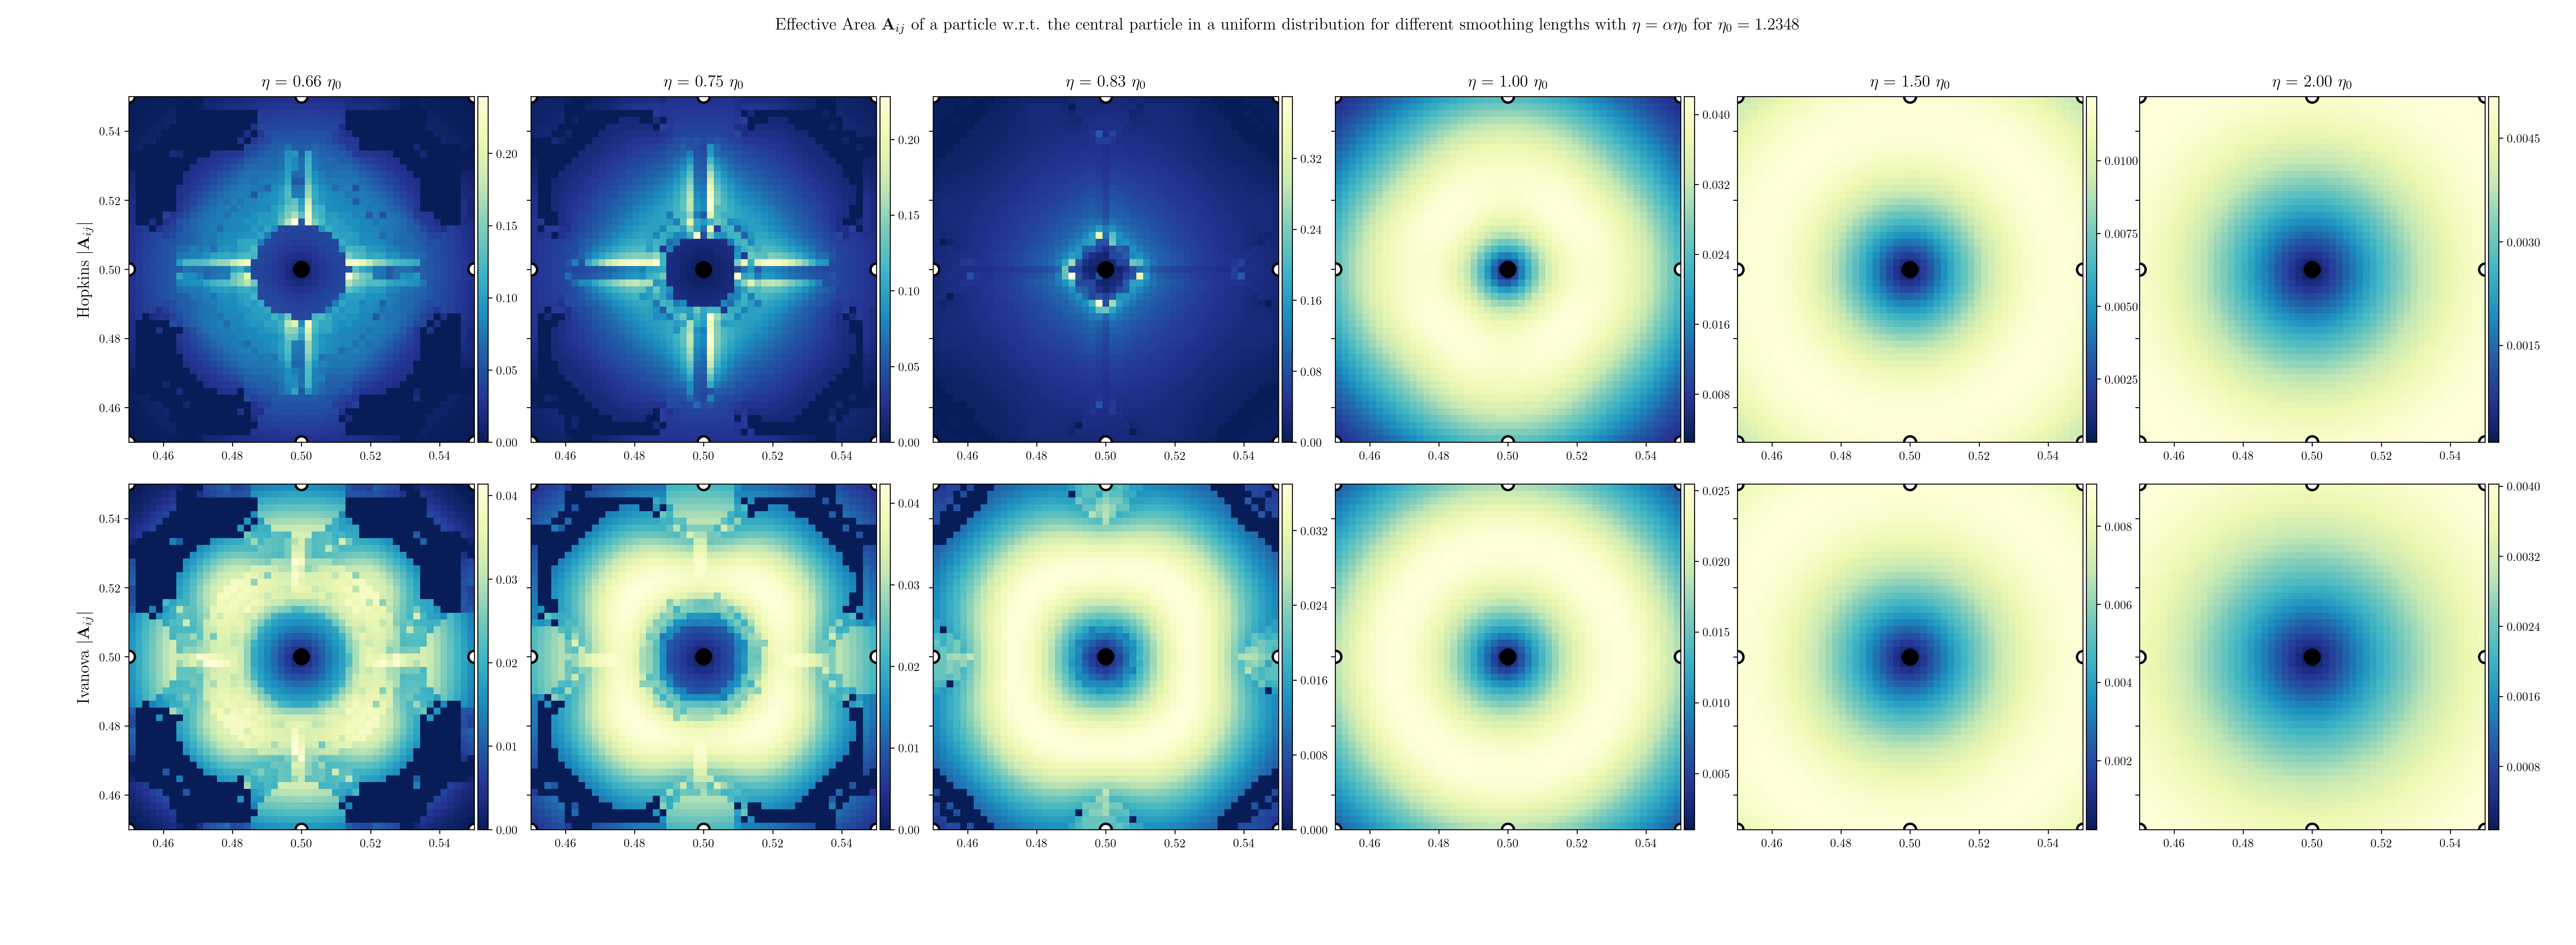
\includegraphics[width=\textwidth]{figures/Meshless/different-smoothing-lengths.png}
% \caption{\label{fig:different-smoothing-lengths}
%     The norm of \Aij\ for both the Hopkins and Ivanova expression for a particle being displaced
% in an otherwise uniform particle configuration w.r.t the central (black) particle for various
% smoothing lengths specified by $\eta$.
%     The white circles show the positions of the closest neighbor particles of the central one.
%     The value of \Aij\ of the displaced particle at a certain point on the plotted plane
% determines that point's color.
% }
% \end{figure}
%
%
%
%
% Figure \ref{fig:different-kernels} shows the \Aij\ for both versions of the expressions for an
% additional particle within uniformly distributed particles for different kernels $W$.
% Again the norm of the computed \Aij\ is plotted at that displaced particles' position.
%
% With different kernels, it is easier to see that the size of the \Aij\ doesn't behave radially
% symmetric in a uniform particle distribution.
% The Hopkins version appears to develop ``crosses'' with higher order kernels used, the Ivanova one
% displays a more rectangular shape.
% Interestingly, the ``rectangles'' for Hopkins and Ivanova seem to be rotated by 45$\degr$.
% An implementation of the Ivanova formula where the gradients aren't computed analytically, but using
% expression \ref{eq:gradient}, shows that this shape of the contours is determined by the gradient
% used.
%
%
%
% \begin{figure}[htpb]
% 	\centering
% 	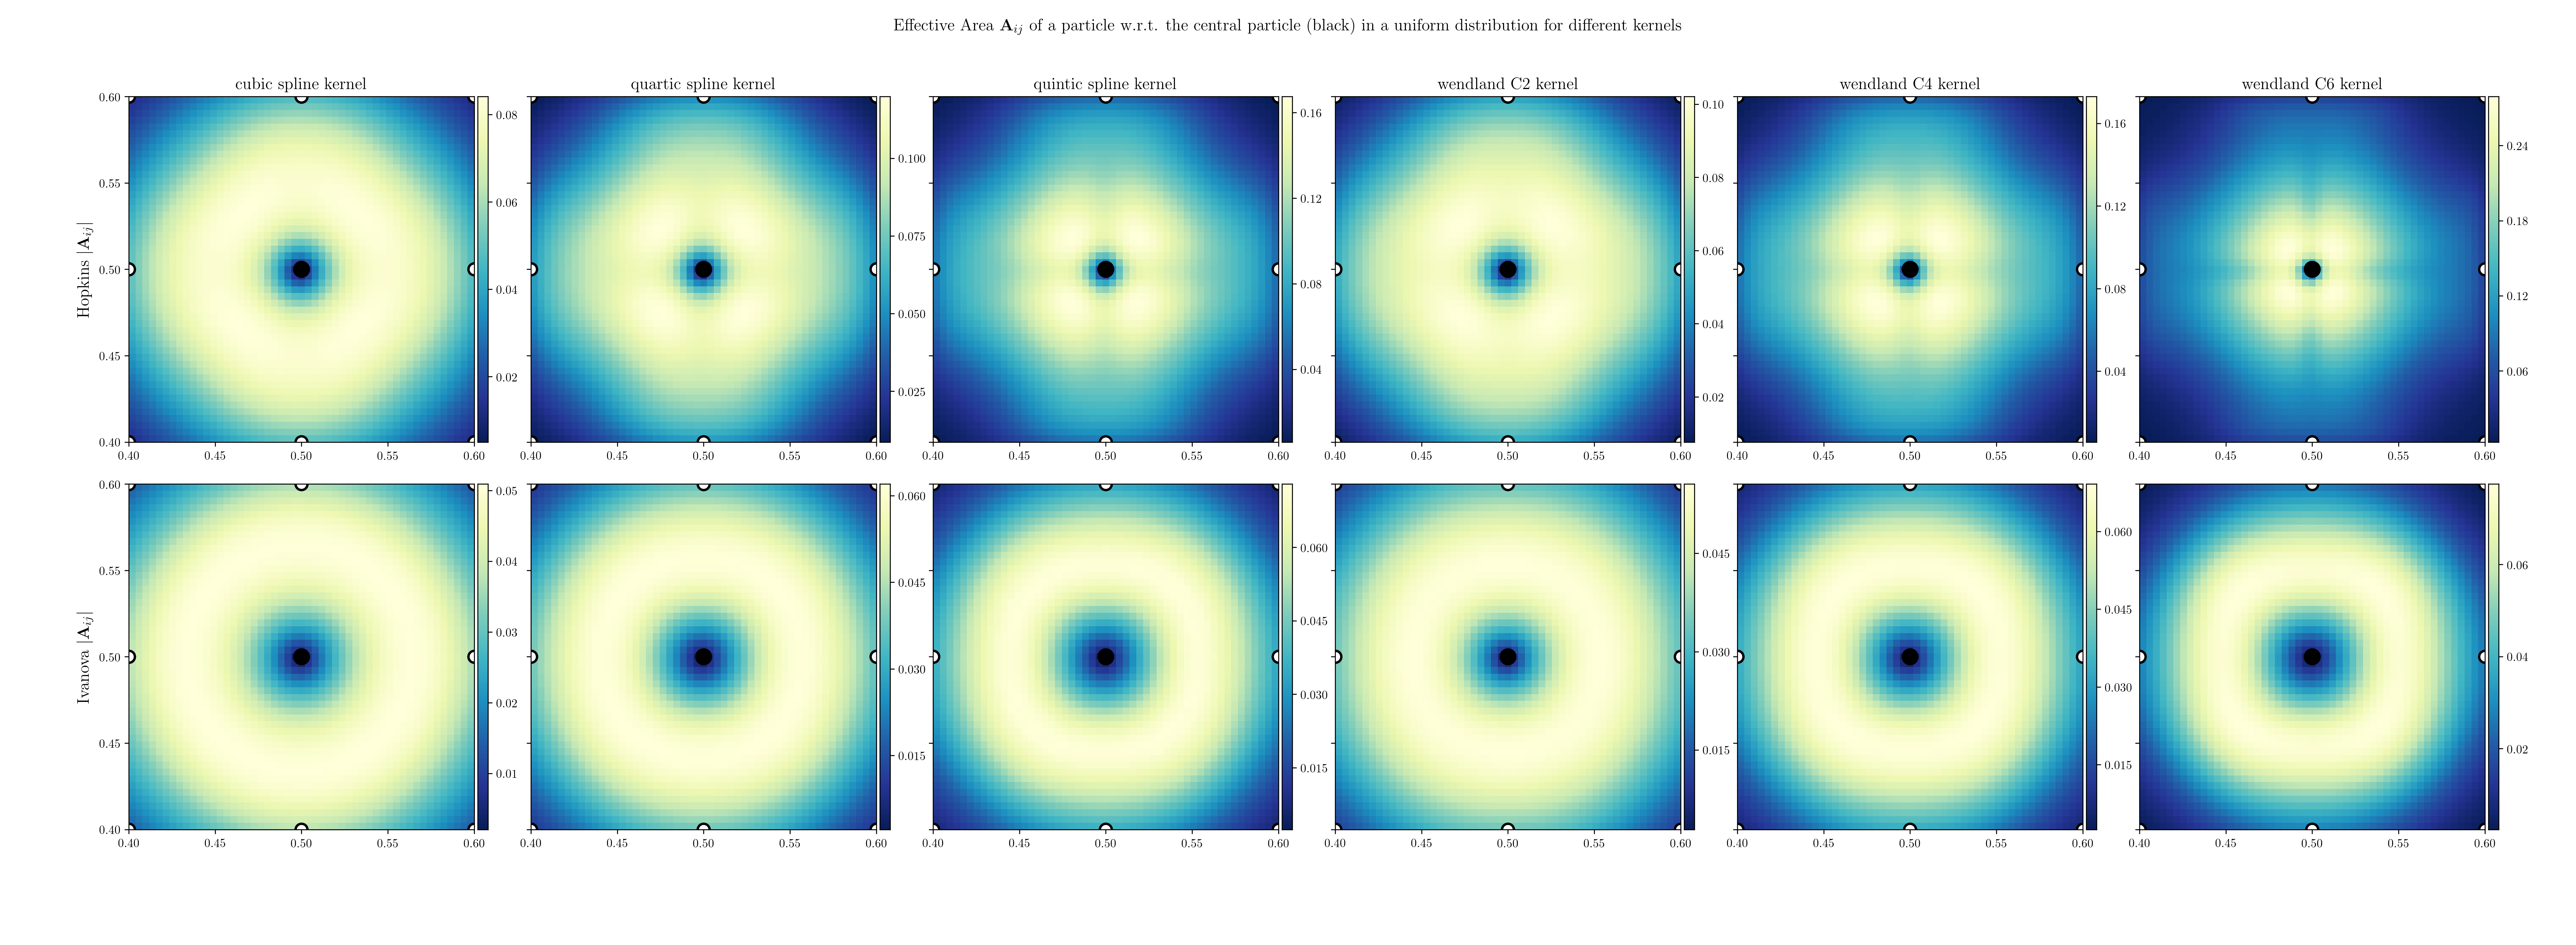
\includegraphics[width=\textwidth]{./figures/Meshless/different-kernels.png}
% 	\caption{\label{fig:different-kernels}
% 		The norm of \Aij\ for both the Hopkins and Ivanova expression for a particle being displaced
% in an otherwise uniform particle configuration w.r.t the central (black) particle for various
% kernels $W$.
% 		The white circles show the positions of the closest neighbor particles of the central one.
% 		The value of \Aij\ of the displaced particle at a certain point on the plotted plane
% determines that point's color.
% 	}
% \end{figure}
%
%








%-------------------------------------
% \subsubsection{Conclusions}
%-------------------------------------

%-----------------------------------------------------------------------
\subsubsection{Summary}
%-----------------------------------------------------------------------


To summarize the findings, there are clear differences in the magnitudes of the \Aij\ obtained
using the Ivanova and Hopkins formulation, with factors up to $\sim 3$.
Not only the magnitudes differ, but the directions of the normal vectors to the surfaces \Aij\ do
as well. The total sum of the norms of \Aij\ of the Ivanova expression is almost always smaller
than the Hopkins version. This could lead to smaller total fluxes and possibly allow bigger time
step sizes when using the Ivanova version. Additionally, the Ivanova methods display a higher
relative contribution with increasing distance from the central particle than the Hopkins method.
This could lead to the method being more diffusive, but simultaneously could also mean that it's
more stable under extreme conditions like violent shocks.

A further advantage of the Ivanova formulation is that the effective surfaces are well-defined even
in troublesome particle configurations. The Hopkins version requires the inversion of a matrix (eq.
\ref{eq:matrix_B}), which can lead to problems if the matrix $\mathcal{B}$ is singular.
In that sense, the Ivanova version could make the hydrodynamics method more stable.











%-------------------------------------------------------------------
\subsection{Comparison in Hydrodynamical Applications}
%-------------------------------------------------------------------

\begin{figure}
    \centering
    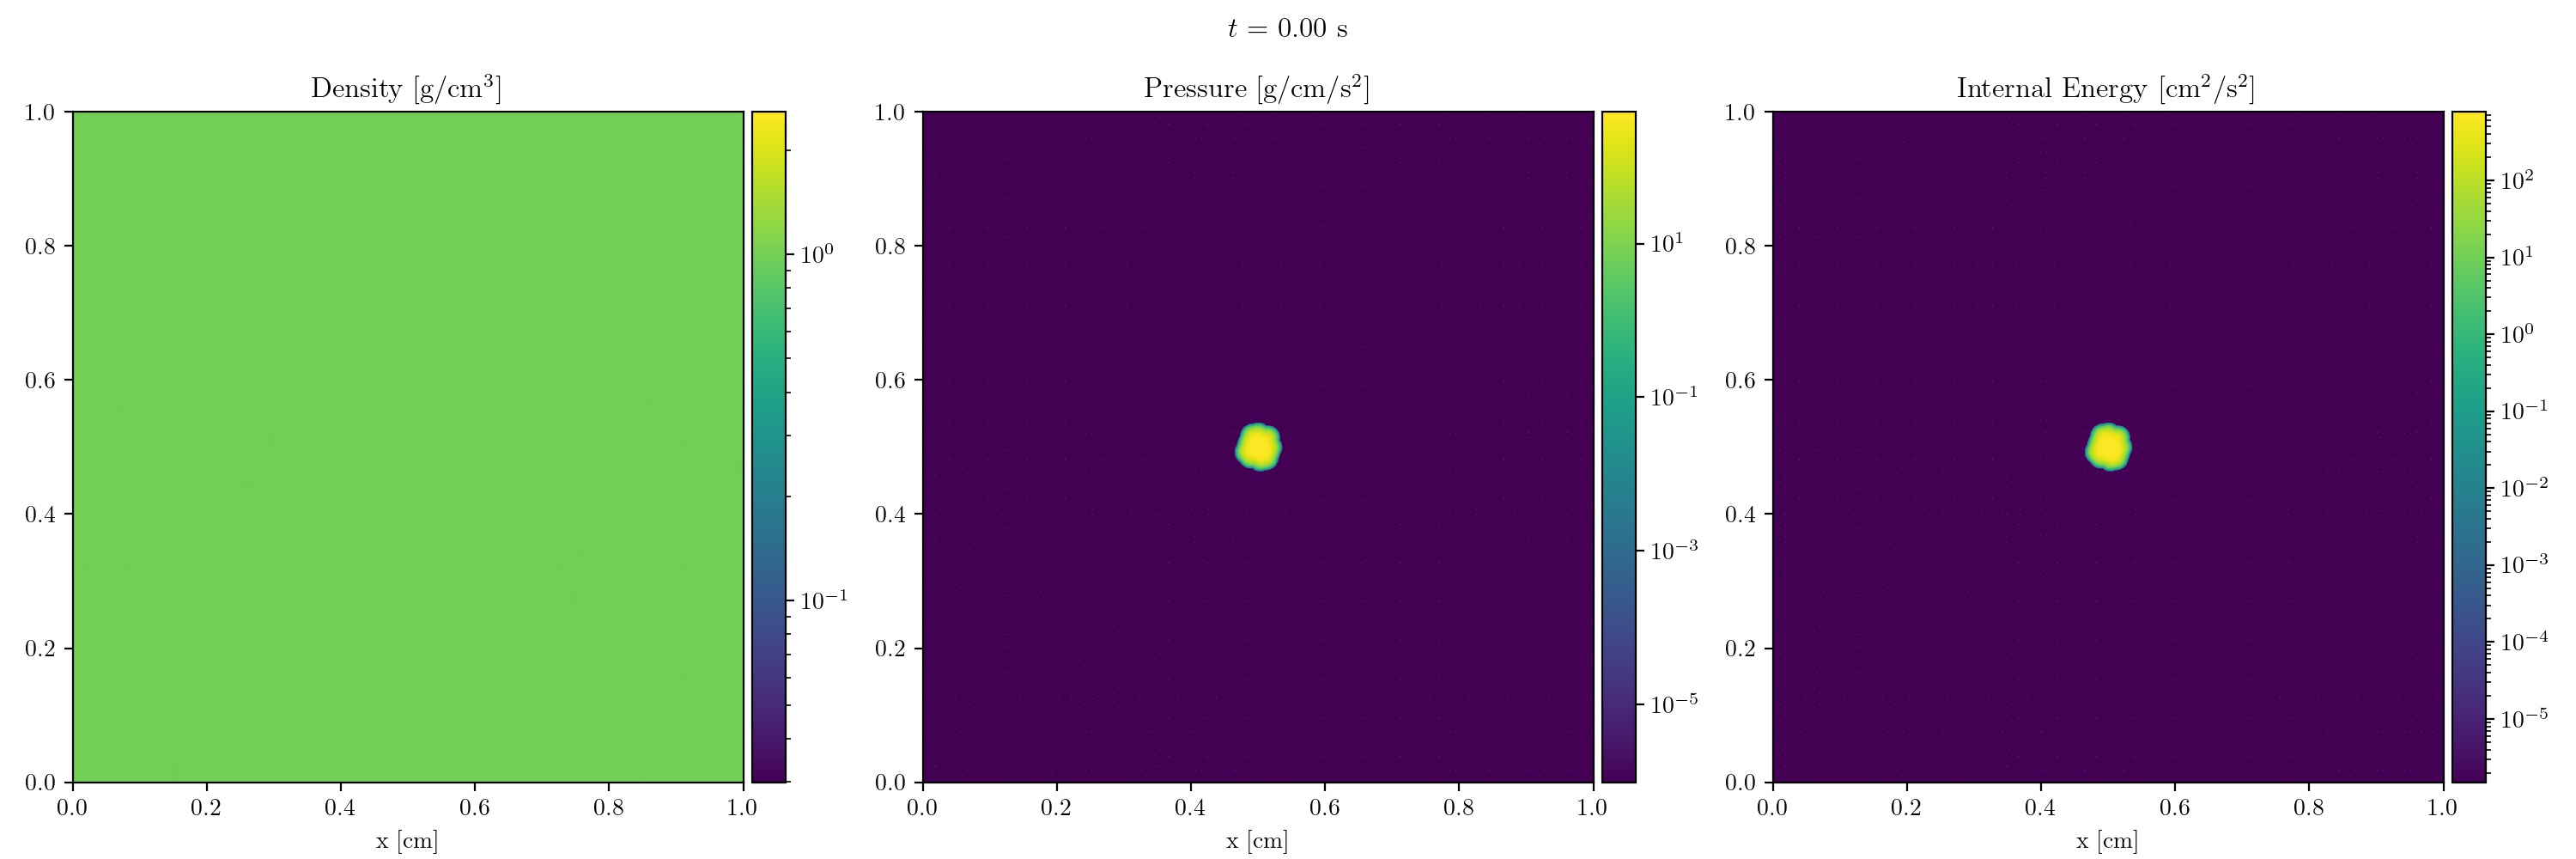
\includegraphics[width=\textwidth]{figures/Meshless/sedov_0000.png}%
\\
    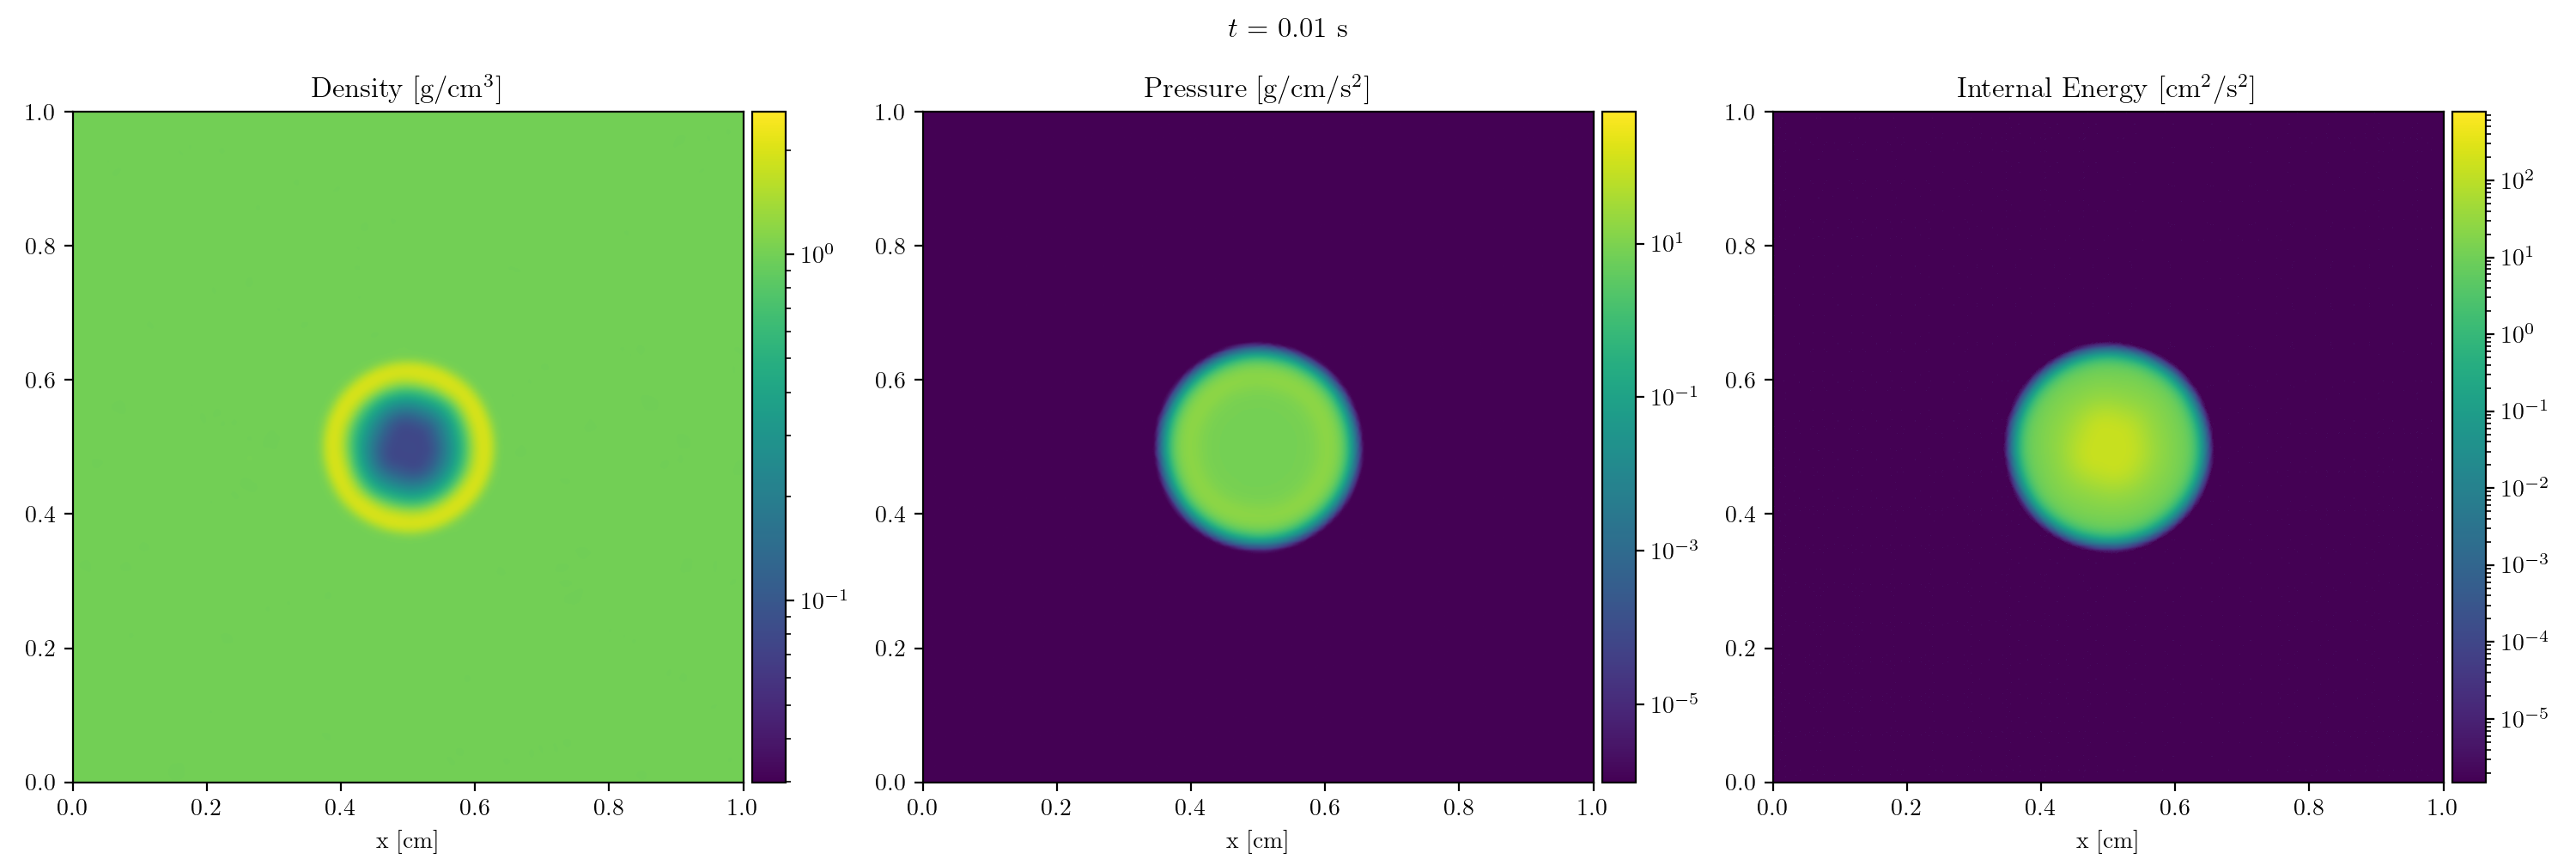
\includegraphics[width=\textwidth]{figures/Meshless/sedov_0001.png}%
\\
    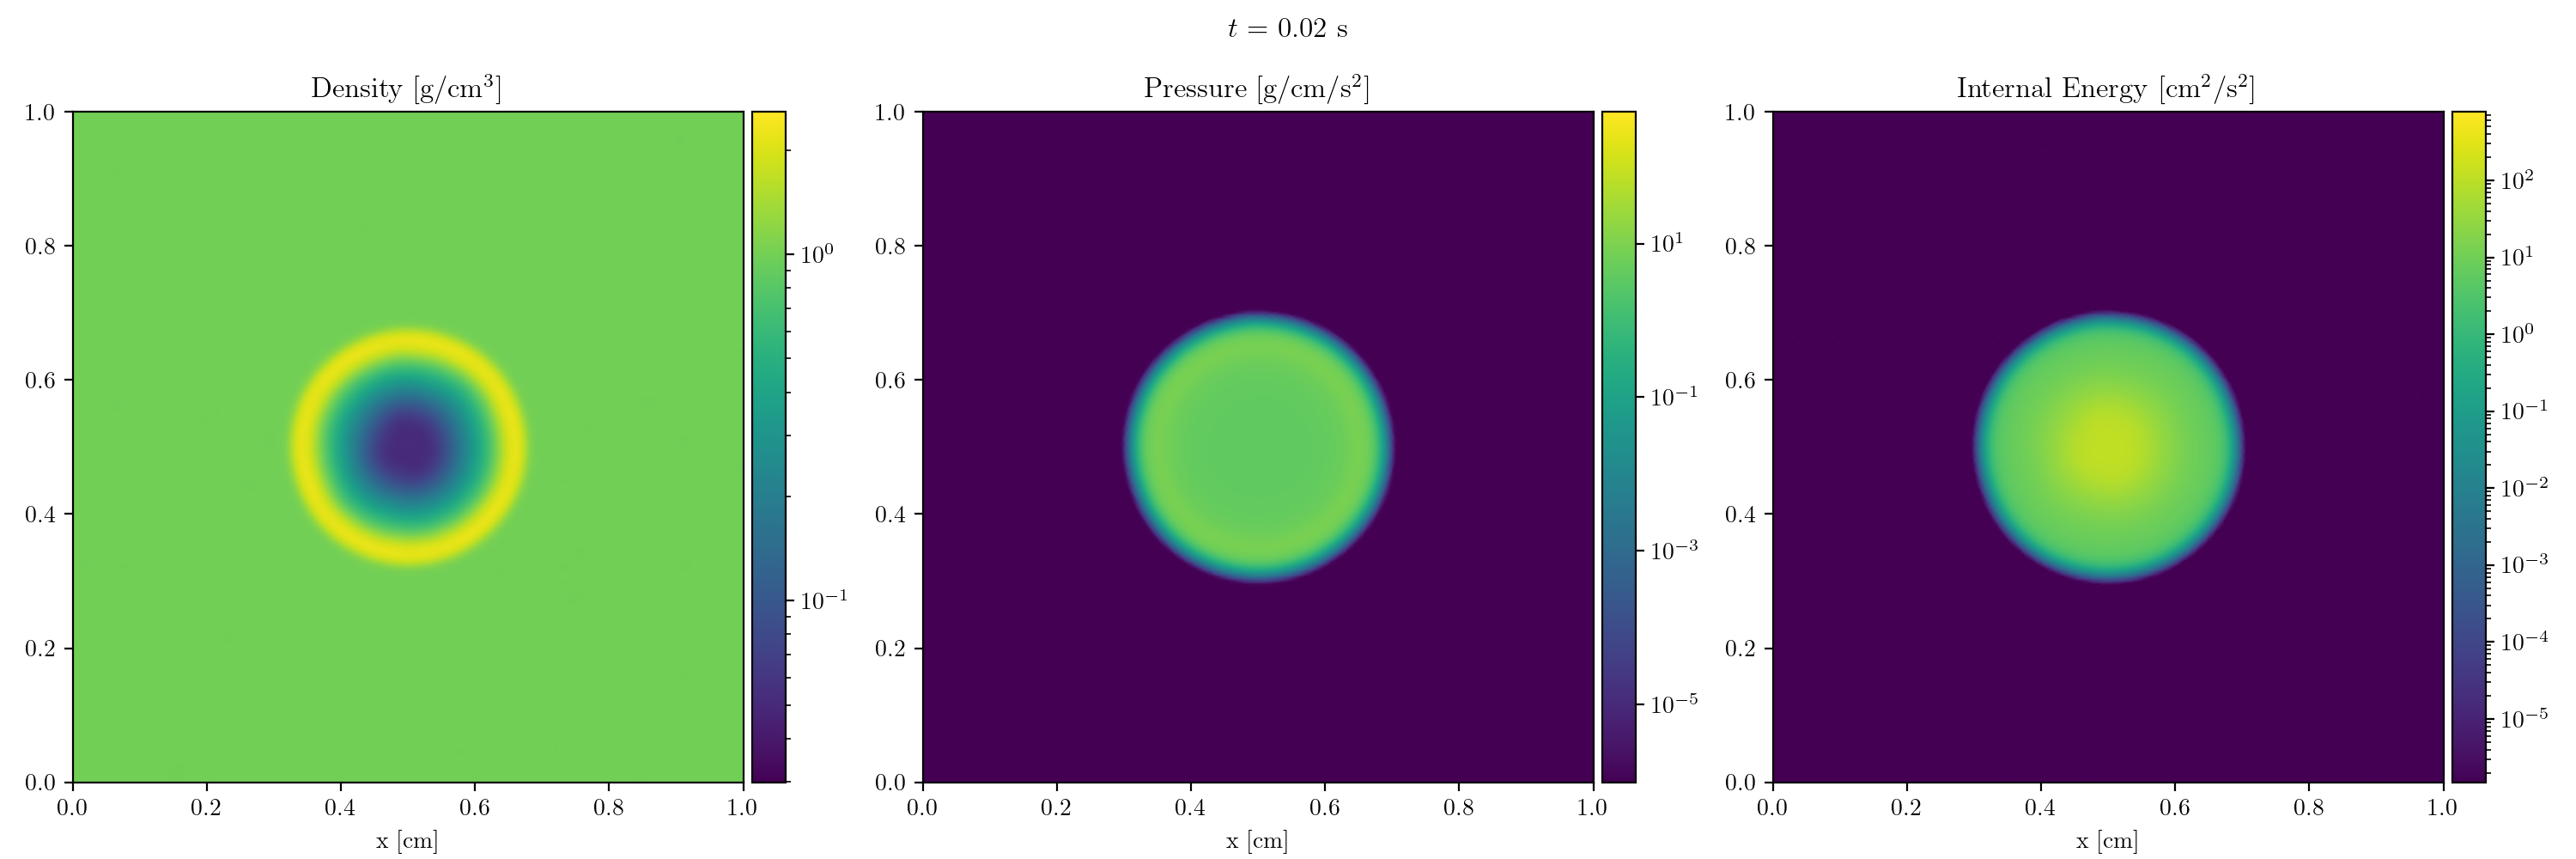
\includegraphics[width=\textwidth]{figures/Meshless/sedov_0002.png}%
\\
    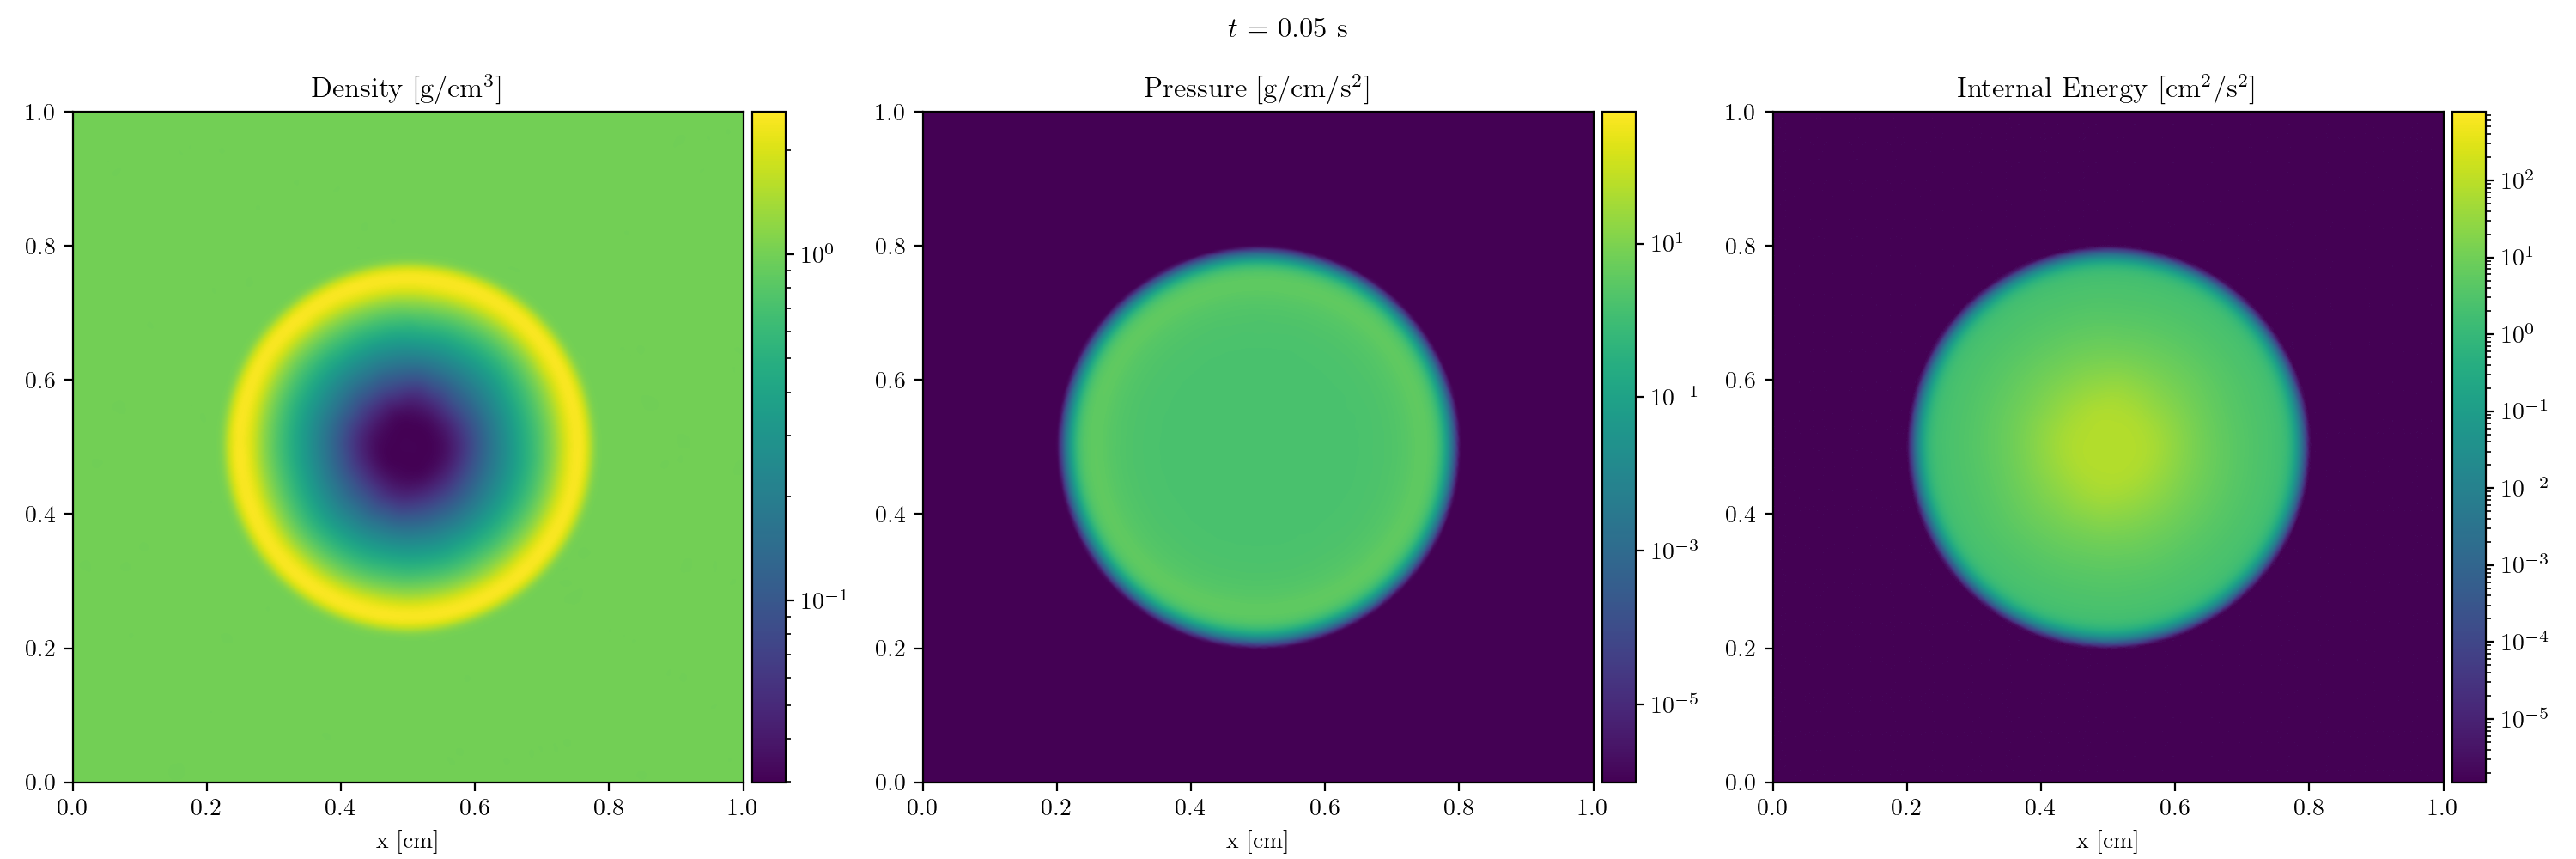
\includegraphics[width=\textwidth]{figures/Meshless/sedov_0005.png}%
    \caption{
The results of the Sedov blast test in two dimensions at times $t = 0.0$s, $0.01$s, $0.02$s, and
$0.05$s for density, pressure, and internal energy. The initial conditions are set up such that a
few particles in the center of the box are injected with a high energy end pressure, which results
in a spherical explosion. The shown solution was obtained using the Hopkins \Aij and while keeping
particles static. Using the Ivanova \Aij with static particles results in a nearly identical
solution, which can be seen in the profiles shown in the top row of
Figure~\ref{fig:hopkins-ivanova-sedov}. These figures were created with the \swiftsimio python
library \citep{borrowSwiftsimioPythonLibrary2020}.
    }
    \label{fig:meshless-sedov-solution}
\end{figure}



\begin{figure}
    \centering
    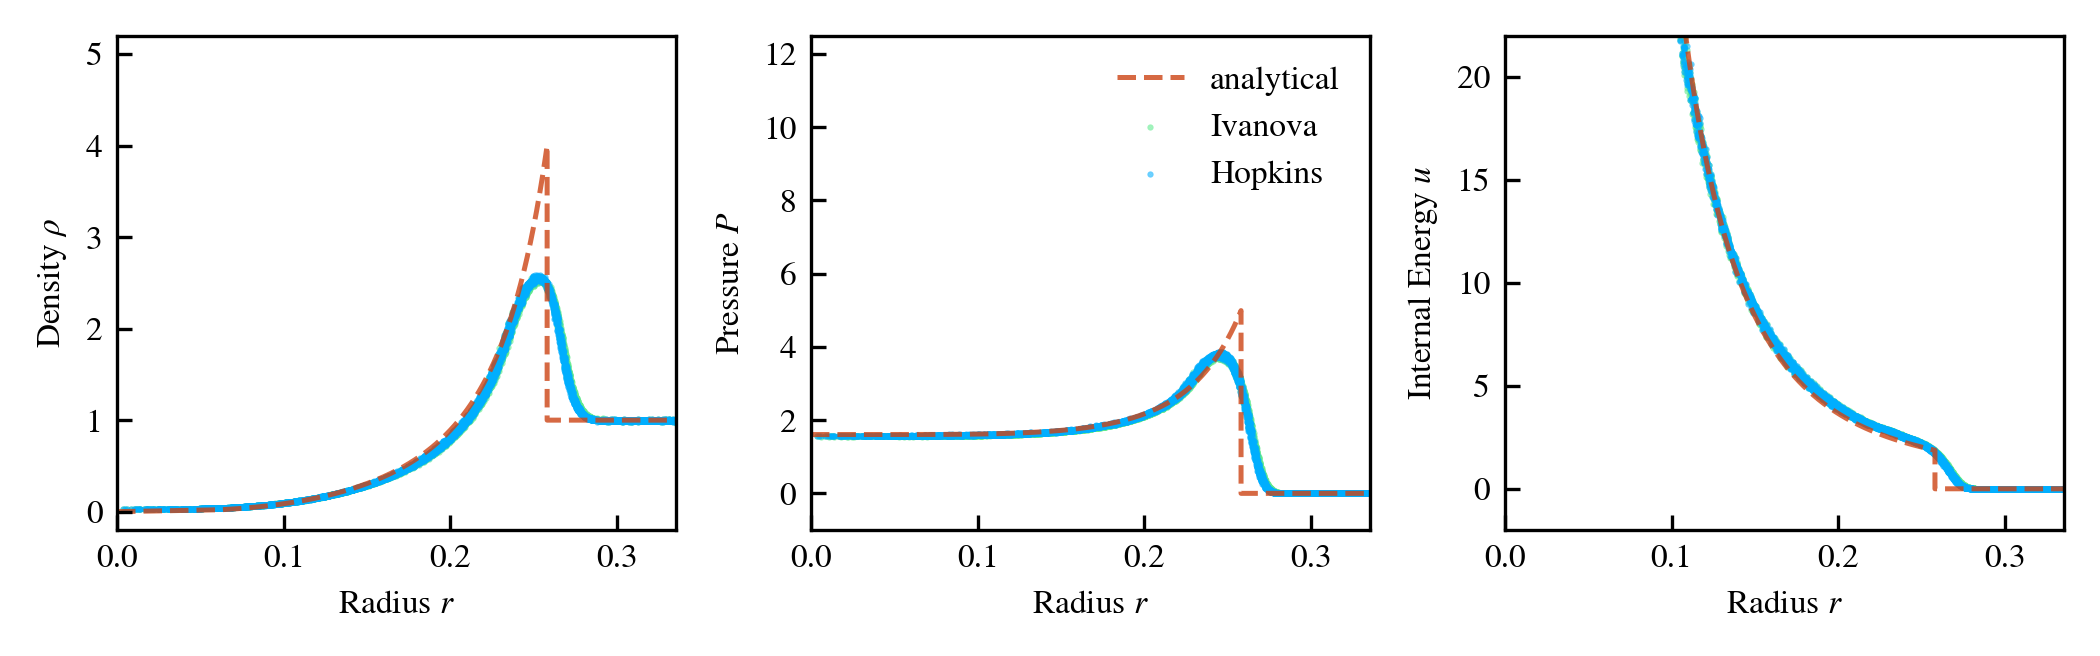
\includegraphics[width=\textwidth]{figures/Meshless/sedov-static.png}%
\\
    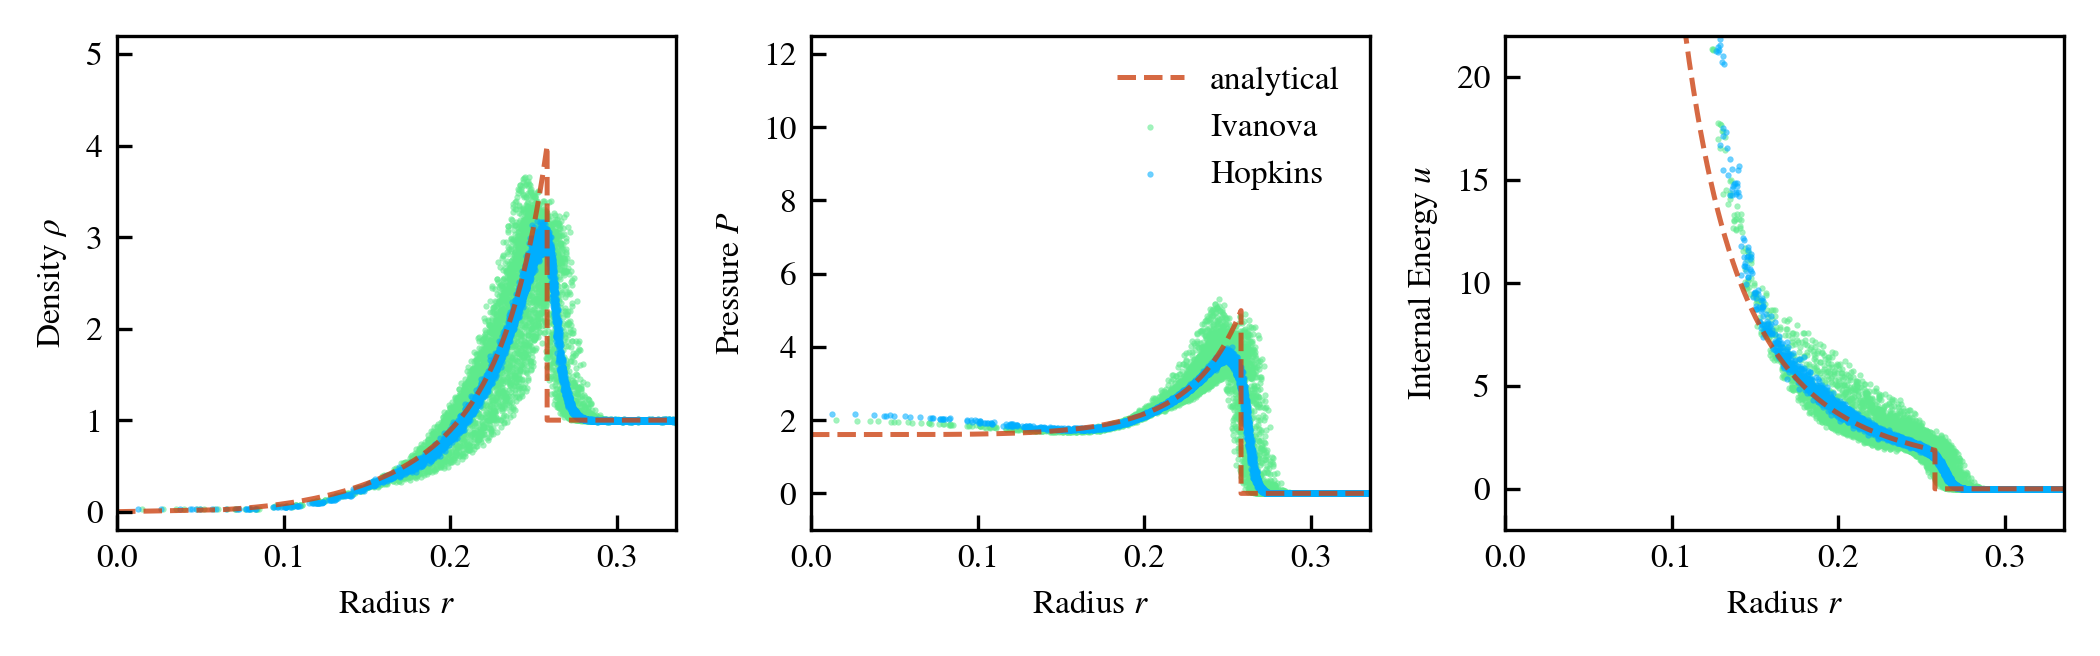
\includegraphics[width=\textwidth]{figures/Meshless/sedov-lagrangian.png}%
    \caption{
A Sedov blast test using both Hopkins and Ivanova effective surface. The blue points are the
solutions using the effective surfaces of \cite{hopkinsGIZMONewClass2015}, the green dots are the
solution using the \cite{ivanovaCommonEnvelopeEvolution2013} \Aij. The density, pressure, and
internal energy are shown as a function of radius from the center, in arbitrary units. The top row
shows the results when particles are kept static, i.e. are not being drifted. The results using
the Hopkins and Ivanova expressions for surfaces \Aij are virtually identical. The bottom row shows
the results for Lagrangian particles. The dashed line shows the analytical solution.
    }
    \label{fig:hopkins-ivanova-sedov}
\end{figure}

\begin{figure}
\minipage{0.33\textwidth}
	\centering
	Initial Conditions
  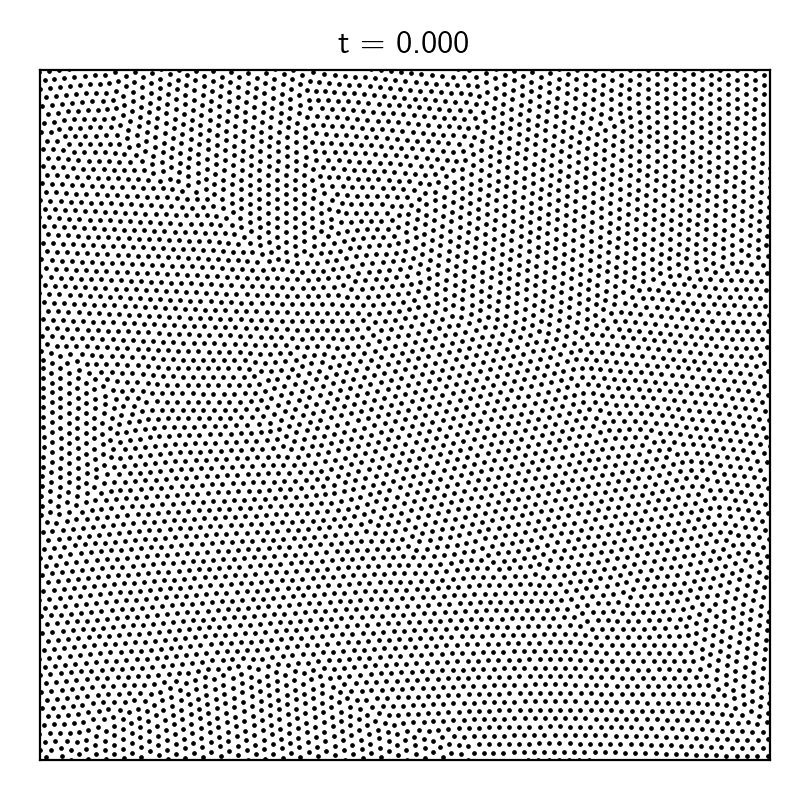
\includegraphics[width=\linewidth]{figures/Meshless/positions_sedov_glass_IC.png}
\endminipage\hfill
\minipage{0.33\textwidth}
	\centering
	Hopkins Solution
  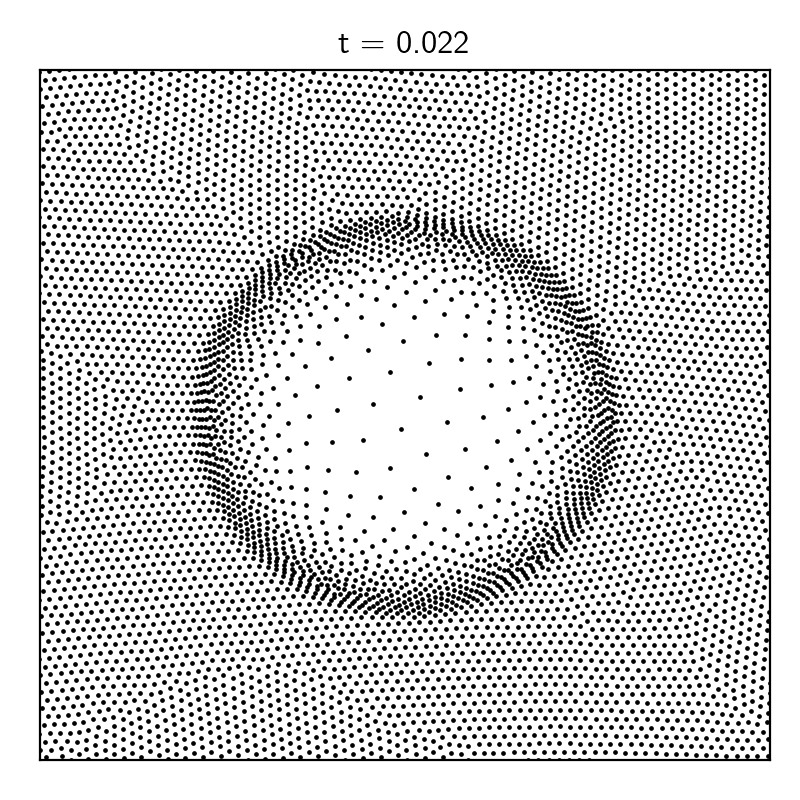
\includegraphics[width=\linewidth]{figures/Meshless/positions_sedov_hopkins_glass.png}
\endminipage\hfill
\minipage{0.33\textwidth}%
	\centering
	Ivanova Solution
  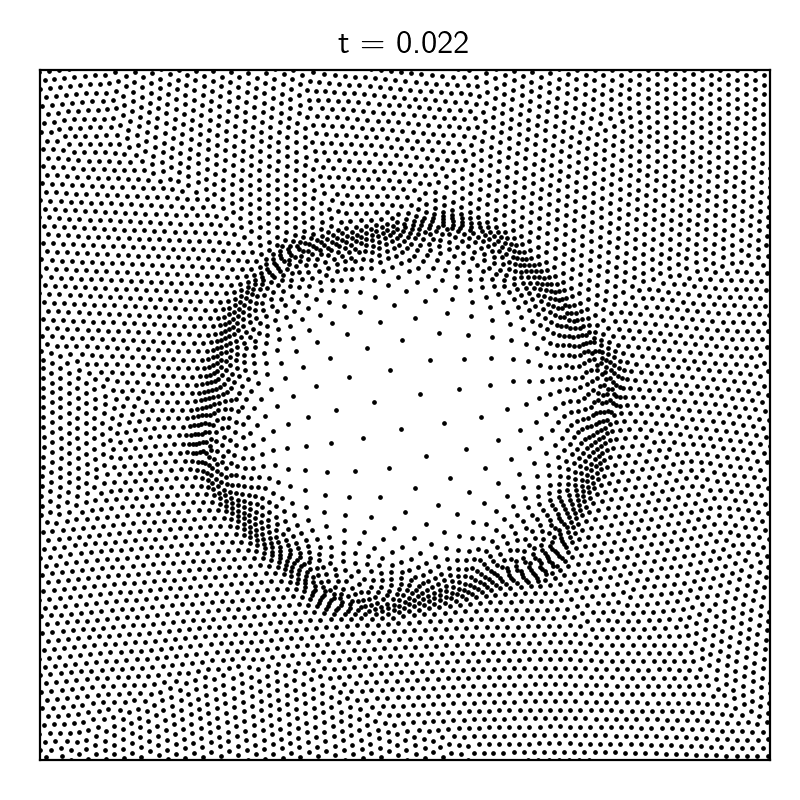
\includegraphics[width=\linewidth]{figures/Meshless/positions_sedov_ivanova_glass.png}
\endminipage\\
%
%
% \begin{figure}[!htb]
\minipage{0.33\textwidth}
  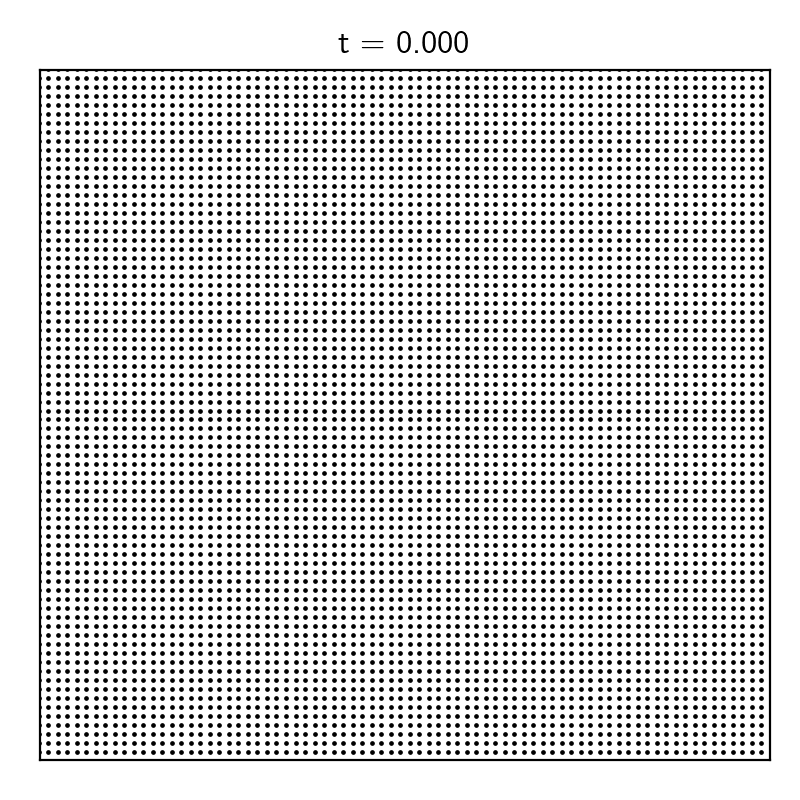
\includegraphics[width=\linewidth]{figures/Meshless/positions_sedov_uniform_IC.png}
\endminipage\hfill
\minipage{0.33\textwidth}
  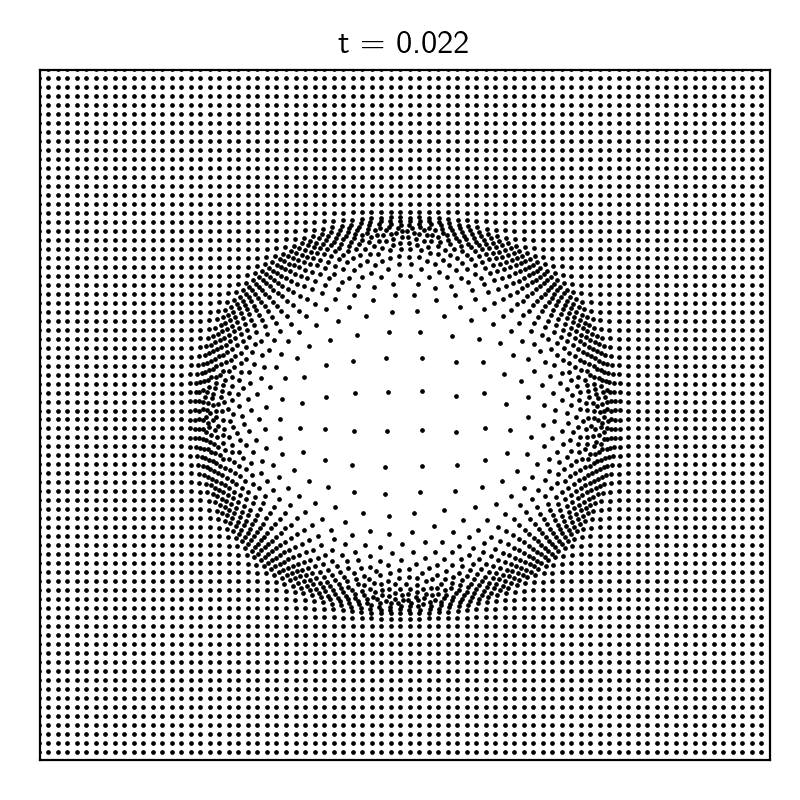
\includegraphics[width=\linewidth]{figures/Meshless/positions_sedov_hopkins_uniform.png}
\endminipage\hfill
\minipage{0.33\textwidth}%
  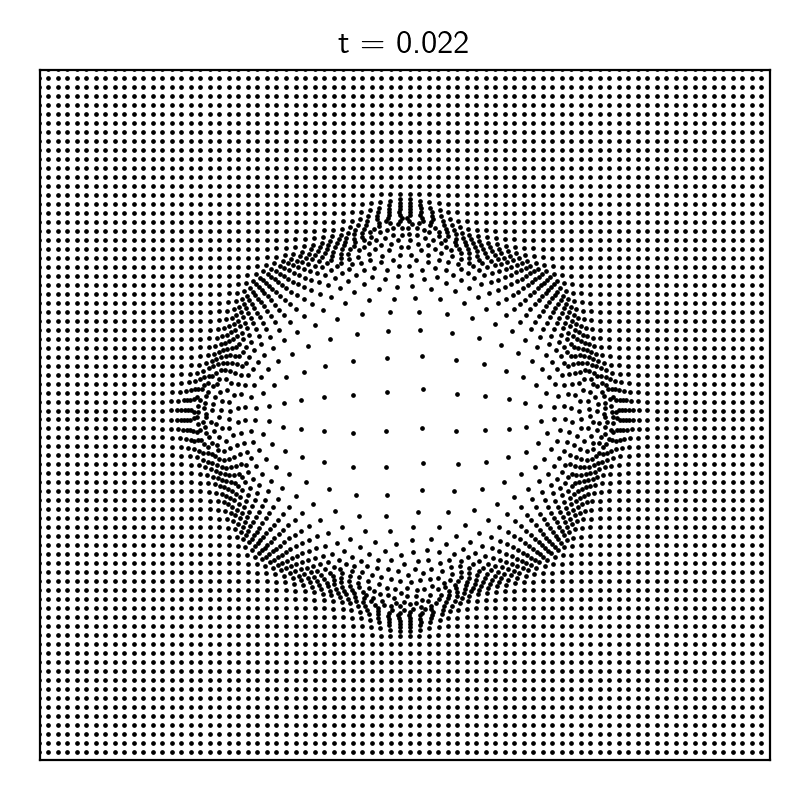
\includegraphics[width=\linewidth]{figures/Meshless/positions_sedov_ivanova_uniform.png}
\endminipage
\caption{
The influence of the initial conditions on the classical Sedov blast test. Plotted are the particle
positions of the initial conditions on the left, the solution provided by the
\citet{hopkinsGIZMONewClass2015} version in the middle and the
\citet{ivanovaCommonEnvelopeEvolution2013} version of the finite volume particle method on the right
for glass like initial particle positions (top) and initially uniformly placed particles (bottom)
for a Sedov blast, in arbitrary length and time units.
The blast should be a radially symmetric explosion from the center, which is well approximated with
the \citet{hopkinsGIZMONewClass2015} version, but not with the Ivanova version. Instead, the shape
of the blast wave is determined by the underlying particle configuration: hexagon-shaped for the
glass initial conditions, and octagon-like for the uniform particle configuration.
  }
\label{fig:sedov-particle-positions}
\end{figure}




\begin{figure}
    \centering
    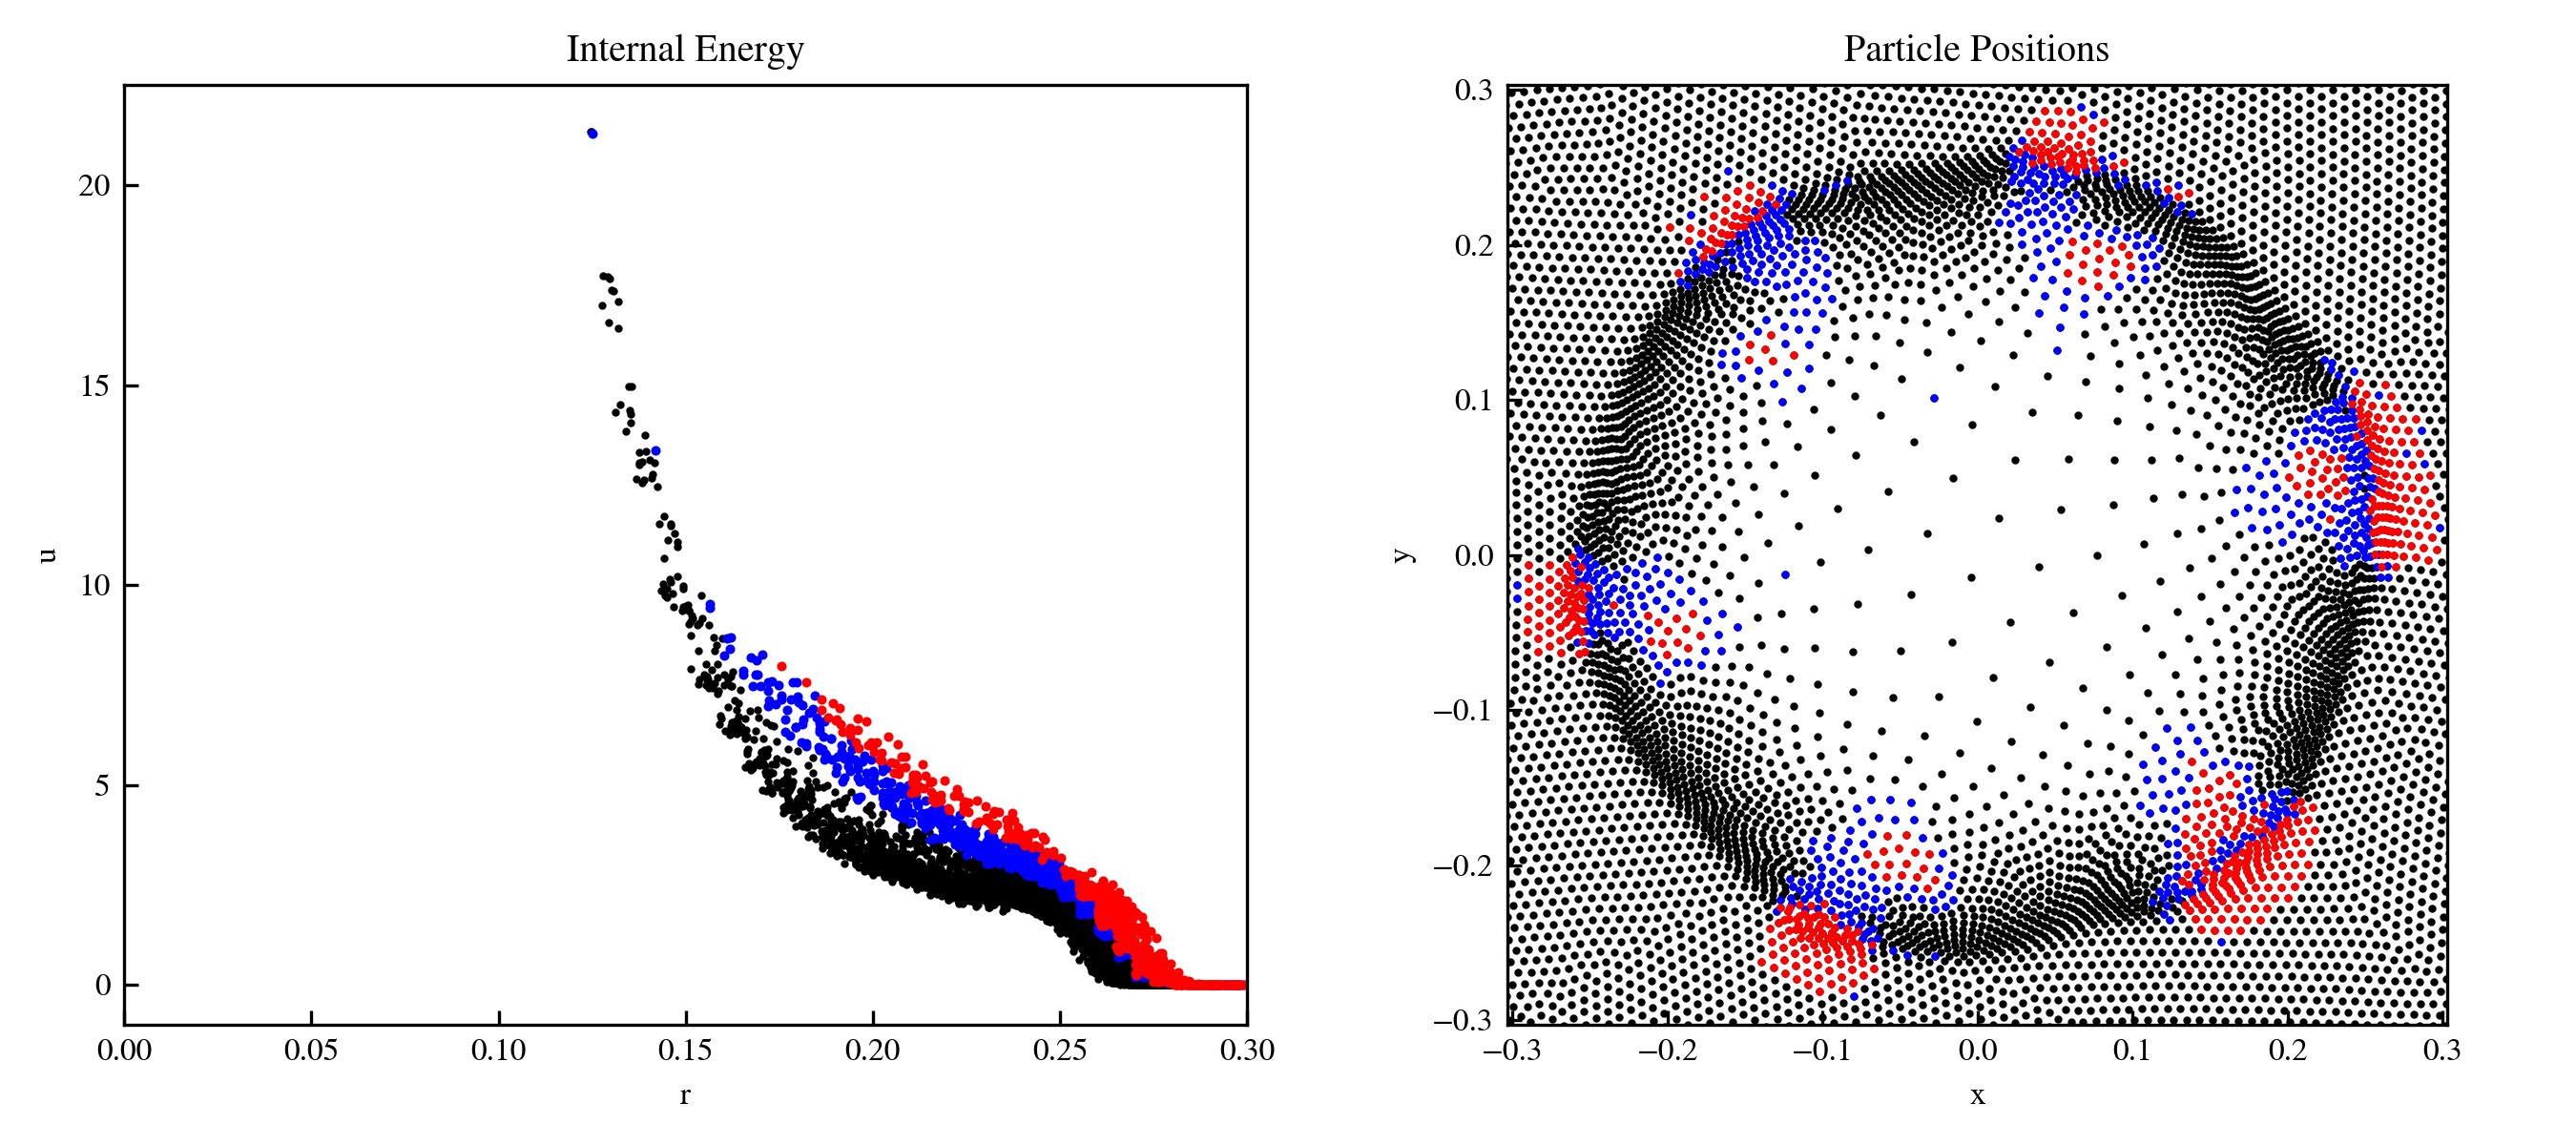
\includegraphics[width=.8\textwidth]{figures/Meshless/sedov-ivanova-marked-particles.png}%
    \caption{
On the left, the internal energy $u$ as a function of radius $r$ from the center of the solution of
the Sedov blast test using the Ivanova \Aij and Lagrangian particles is shown. The output is
performed at the same time as in Figure~\ref{fig:hopkins-ivanova-sedov}. Particles with internal
energies above 1.2 and 1.5 times the average internal energy at that radius are marked blue and
red, respectively. On the right, the particle positions of the solution at the same time are shown.
The blue and red particles are the same particles marked correspondingly in the left plot,
highlighting that the scatter seen in the left plot and in Figure~\ref{fig:hopkins-ivanova-sedov}
are in regions where the particle configuration has become irregular and deformed following the
initial glass-like configuration.
    }
    \label{fig:sedov-ivanova-marked}
\end{figure}


To conclude the comparison between the Hopkins and Ivanova versions of FVPM, let's look at their
performance on actual hydrodynamical tests. The experiments are run using the simulation code \swift \citep{schallerSWIFTSPHInterdependent2018a}, which contained an implementation of the Hopkins version outlined in Section~\ref{chap:meshless-full} already, but not the Ivanova one yet. The details of the implementation will be discussed in detail later in Chapter~\ref{chap:meshless-implementation}.

Running actual hydrodynamics tests with both method revealed that the Ivanova formulation has some
big trouble when applied on Lagrangian particles. Figure~\ref{fig:hopkins-ivanova-sedov} shows the
solution to a classical test, the Sedov blast, in two dimensions. The initial conditions are set up
such that a few particles in the center of the box are injected with a high energy end pressure,
which results in a spherical explosion. When running the simulation as an Eulerian code, i.e.
keeping particles static, the results are nearly identical for both versions of effective surfaces
\Aij. The results are somewhat diffusive, which is to be expected since the interacting particle
pairs are spread out over a larger region compared to what a grid code that only interacts adjacent
cell pairs would require. Moving the particles along with the fluid however introduces a very strong scatter in the solution using the Ivanova \Aij, while the Hopkins version delivers adequate results.
The reason for the scatter appears to be a strong dependency of the Ivanova \Aij on the particle
configuration. Figure~\ref{fig:sedov-particle-positions} shows the particle positions for two
different underlying initial configurations: a glass-like ordering, and a uniform configuration. In
both cases the evolution of the blast wave with the Ivanova \Aij shows strong traces of the initial
particle positions. Figure~\ref{fig:sedov-ivanova-marked} shows the result of the Sedov blast with
the Ivanova \Aij where some particles are marked based on their internal energy $u$. It is clear
that the strong scatter is introduced by the deformities that follow the underlying initial particle configuration.

The same issues with the Ivanova surfaces appears for a wide variety of other tests. Unfortunately
neither a different choice of kernels, nor increasing the number of neighbors for particles to
interact with, nor very small Courant numbers, nor using much more restrictive limiters were able to alleviate the problem noticeably. This leads to the conclusion that in the presented form, the
Ivanova version of the finite volume particle method is not suitable for ``real life'' application
for hydrodynamics in the astrophysical and cosmological context. \footnote{
However, the Ivanova version appears to be an adequate choice for applications which don't require
co-moving particles, as is for example the case for the transport of radiation, which will be the
topic in Part~\ref{part:rt} of this thesis.}.
Having Lagrangian particles is absolutely necessary for cosmological simulations, and the Ivanova
\Aij do not work well with co-moving particles. A possible solution would be to determine the
particle velocities with a different method than the one used to evolve the fluid quantities. For
example, the particle velocities could be set using the results of a simple first order accurate
method, or using some basic SPH formulation, both of which typically aren't very sensitive to the
underlying particle configuration. Testing these solution attempts remains a subject for future
works.





